
\documentclass[12pt]{report}
\usepackage[ansinew]{inputenc}
\usepackage[T1]{fontenc}
\usepackage{latexsym}
\usepackage{fixltx2e}
\usepackage[lofdepth,lotdepth]{subfig}
\usepackage{graphicx,epstopdf}
\usepackage[absolute]{textpos}
\usepackage[english]{babel}
%\usepackage[latin1]{inputenc}
\usepackage{amsmath,amsfonts}
\usepackage{natbib}
\usepackage{fancyhdr}
\usepackage{wrapfig}
\usepackage{float}
\usepackage[Conny]{fncychap}
\usepackage[usenames,dvipsnames]{color}
\usepackage{color, colortbl}
\usepackage{longtable}
\usepackage{multirow}
\usepackage{algorithmic}
\setcitestyle{numbers,open={[},close={]}}
\usepackage{epsfig}
\usepackage[official,right]{eurosym}
\usepackage{rotating}
\usepackage{hyperref}
\usepackage{rotating}
\hypersetup{pdfborder={0 0 0}}
\usepackage[absolute]{textpos}
\usepackage[rounded]{syntax}
\usepackage{appendix}
\grammarparsep 1pt
\usepackage{xyling}
\usepackage{pdfpages}

\usepackage{slashbox}
\usepackage{verbatim}
\usepackage{float}

\newfloat{Code}{H}{myc}
\allowdisplaybreaks


% Color definitions
\definecolor{light-gray}{gray}{0.95}
% Color definitions


%EPS images snask

%\usepackage{epstopdf}

\newif\ifpdf
\ifx\pdfoutput\undefined
   \pdffalse
\else
   \pdfoutput=1
   \pdftrue
\fi
\ifpdf
   \usepackage{graphicx}
   \usepackage{epstopdf}
   \DeclareGraphicsRule{.eps}{pdf}{.pdf}{`epstopdf #1}
   \pdfcompresslevel=9
\else
   \usepackage{graphicx}
\fi
%eps image snask end
\epstopdfsetup{suffix=}

%semantic udtryk
\usepackage{turnstile}
%$\nststile{Bottom}{Top}$

%\usepackage[tt]{titlepic}


%LOL MARTIN!
%End lool martin

% C# lol?
\usepackage{listings}
% default words comes from lstlang1.sty
\lstset{language=Java,
  basicstyle=\ttfamily\footnotesize\bfseries,
  float,
  columns=flexible,
  morekeywords=[1]{TmdbAPI,TmdbMovie},
  %keywordstyle=[1]\sffamily,
  backgroundcolor=\color{light-gray},
  captionpos=b,
  frame=single,
  breaklines=true, 
  keywordstyle=\color{Blue},
  commentstyle=\color{Green},
  stringstyle=\color{Mahogany},
  showspaces=false,
  showstringspaces=false,
  numbers=left,                   % where to put the line-numbers
  numberstyle=\footnotesize,      % the size of the fonts that are used for the line-numbers
  stepnumber=1
  }  \newenvironment{program}


% Code environment definition --- Java
% Usage 1: \lstinputlisting[style=sw6Java,label=something,caption=Tove]{someFile or someActualCode}   --- is shown in \listoflistings
% Usage 2: \lstinline[style=sw6Java]{someCode}   --- is not shown in \listoflistings
\lstdefinestyle{sw6Java} {
  language=Java,
  basicstyle=\ttfamily\footnotesize\bfseries,
  float,
  columns=flexible,
  morekeywords=[1]{TmdbAPI,TmdbMovie},
  %keywordstyle=[1]\sffamily,
  backgroundcolor=\color{light-gray},
  captionpos=b,
  frame=single,
  breaklines=true, 
  keywordstyle=\color{Blue},
  commentstyle=\color{Green},
  stringstyle=\color{Mahogany},
  showspaces=false,
  showstringspaces=false,
  numbers=left,                   % where to put the line-numbers
  numberstyle=\footnotesize,      % the size of the fonts that are used for the line-numbers
  stepnumber=1
}

% Code environment definition --- Java

\usepackage{url}

\definecolor{javared}{rgb}{0.6,0,0} % for strings


\definecolor{javagreen}{rgb}{0.25,0.5,0.35} % comments

\definecolor{javapurple}{rgb}{0.5,0,0.35} % keywords

\definecolor{javadocblue}{rgb}{0.25,0.35,0.75} % javadoc

 
\usepackage{url}%% Define a new 'leo' style for the package that will use a smaller font.
\makeatletter
\def\url@leostyle{%
  \@ifundefined{selectfont}{\def\UrlFont{\sf}}{\def\UrlFont{\small\ttfamily}}}
\makeatother
%% Now actually use the newly defined style.
\urlstyle{leo}


\pagestyle{fancy}
\lhead{}

\newcommand{\code}[1]{\texttt{#1}}
\newcommand{\secref}{section \ref}
\newcommand{\appref}{appendix \ref}
\newcommand{\chapref}{chapter \ref}
\newcommand{\figref}{figure \ref}
\newcommand{\tabelref}{table \ref}
\newcommand{\listref}{listing \ref}
\renewcommand{\headrulewidth}{0.4pt}
\renewcommand{\footrulewidth}{0.4pt}

%Rasmus' kind of lol
\makeatletter
\newenvironment{Figure}{%
\par\addvspace{12pt plus2pt}%
\def\@captype{figure}%
}{%
\par\addvspace{12pt plus2pt}%
}%
\long\def\@makecaption#1#2{%
\vskip\abovecaptionskip
\sbox\@tempboxa{#1: #2}%
\ifdim \wd\@tempboxa >\hsize
#1: #2\par
\else
\global \@minipagefalse
\hb@xt@\hsize{\hfil\box\@tempboxa\hfil}%
\fi
\vskip\belowcaptionskip}
\makeatother
% Rasmus' kind of lol - stop

\setlength{\headheight}{15pt}

%titlepage image halløj
%\usepackage{eso-pic}
%\newcommand\BackgroundPic{
%\put(0,0){
%\parbox[b][\paperheight]{\paperwidth}{%
%\vfill
%\centering
%\includegraphics[width=\paperwidth,height=\paperheight,keepaspectratio]{Images/front-page.png}%
%\vfill
%}}}
%halløj end


%Jesper Stuff

\lstset{
	language=SQL,
  breaklines=true,                                     % line wrapping on
  frame=ltrb,
  framesep=5pt,
  basicstyle=\normalsize,
  keywordstyle=\ttfamily\color{OliveGreen},
  identifierstyle=\ttfamily\color{CadetBlue}\bfseries,
  commentstyle=\color{Brown},
  stringstyle=\ttfamily,
  showstringspaces=false
}

\usepackage[shortlabels]{enumitem}




\title{insert title here} %TODO
\author{os} %TODO

\begin{document}
\maketitle
\tableofcontents
	
	\chapter{Introduction}
In order to describe the context of the system, we -- as a multi project group -- will in the following state the motivation of the project, the group of people we are aiming at helping, the technological platform chosen, the used development method, followed by a problem definition, a system description and architecture, and the conducted usability test.

\section{Motivation}
As this is a student report written as part of a learning project, we are required to comply with the study regulation.
The main areas of focus, according to the study regulation, are: multi project management and quality assurance in the form of requirements analysis, requirements management, and testing.
The goal is to create a comprehensive software system, across multiple project groups, in order to enhance our competences in analysis, design, implementation, and evaluation of software applications in regards to the system requirements\cite{studyreg}.

This project builds on top of a previous project, and is further developed, with the aim of having other students continue the development.
The goal of the project, we are building on top of, is to create a touch based tablet system to support children and their guardians in everyday scenarios.

\section{Target Group}
Our target group is both children and their guardians. These guardians have certain needs for special tools and gadgets that help to ease the communication between them and the children.

Five teachers and educators, who work with children, act as customers. They will provide requirements and information about the institutions' way of working to give us an insight into their daily struggles.

\subsection{Working with Children with ASD}
This section is based upon the statements of a woman with ASD \cite{autism.com}, explaining what it is like to live with ASD, and an interview with an educator at Birken, a special kindergarten for children (see \autoref{InterviewMette} for interview notes).

	People with ASD are often more visual in their way of thinking. Rather than visualizing thoughts in language and text, they do it in pictures or visual demonstrations. Pictures and symbols are therefore an essential part of the daily tools used by children and the people interacting with them. Also, children can have difficulties expressing themselves by writing or talking, and can often more easily use electronic devices to either type a sentence or show pictures, to communicate with people around them.
	Another characteristic of children is their perception of time. Some of them simply do not understand phrases like ``in a moment'' or ``soon'', they will need some kind of visual indicator that shows how long time they will have to wait.

Different communication tools for children with autism already exist, but many of them rely on a static database of pictures, and often these has to be printed on paper in order to use them as intended. Other tools, such as hourglasses of different sizes and colors, are also essential when working with children, and these tools are either brought around with the child, or a set is kept every place the child might go, e.g. being at an institution or at home.

There exists tools today which helps the guardians in their daily life, although -- as stated in Drazenko's quote -- none of them are cost-effective enough to be used throughout the institutions. From the quote, it is clear that there is a need for a more cost-effective solution.

\begin{quotation}
The price of the existing solutions are not sufficiently low such that we can afford to buy and use them throughout the institution.\\ 
	\begin{flushright}
		- Drazenko Banjak, educator at Egebakken.
	\end{flushright}
\end{quotation}

\section{Target Platform}
In this learning project we are developing applications, for children with autism, using the android platform. The android platform was chosen because this project is part of a multi project, which began the development of the Giraf system.\cite{SW6Android2012}\\
---The initial decision decision to work with the android platform seems to be based on the availability of mobile devices to the students.\cite{adminreport}
However, with the budget supplied by AAU, we had the opportunity to exchange the hardware used in the 2011 6'th semester reports, however this has not included smart phones.\\
In selecting a new tablet we had to make considerations:
\begin{itemize}
	\item Popularity of the tablet type can help in distributing the system. Both among early adapters and potential customers.
	\item Accessibility of the OS is a big factor, whether or not we can construct a system on it.
	\item Design and Variety of the physical tablet can figure in.
\end{itemize}
As seen in figure\ref{fig:QuarterlySales}, the two leading operating systems for mobile devices are Apple's iOS and Google's Android.
Being the more widespread of the two, Apple's iOS tablet, the iPad could have been a viable candidate to replace android tablets based entirely on popularity.\\
However, there are some limitations when developing for iOS.
For one, the iOS Development Environment Xcode currently only runs on Macintosh computers, compared to Android that can use the more universal Eclipse environment.\cite{developApple}\cite{androidDevelopers}\\
There are also only 3 variants of the iPad, where two are earlier variants of the latest design, as apple has a monopoly on developing for iOS.
Android Tablets are far more diverse, having many different manufacturers such as HTC\cite{htcflyer}, Samsung\cite{galaxytabs} and Medion.\cite{mediontablet}
The more variety in manufacturers, will allow us to shop around for the best possible fit.\\
All this is overshadowed by that transforming the system into iOS would most likely leave very little time to create new features.\\

We decided to stay with android, but to  upgrade to version 3.2\cite{android32}. 
This version has been chosen because, it is the first version developed mainly for tablets, and it is going to be supported for the duration of the project.
So ordering several Samsung Galaxy Tablets 10.1, based on its larger screen, the android 3.2 OS and the apparent good results the last semester group had with the older Samsung Tablets.---

\begin{figure}
	\centering
		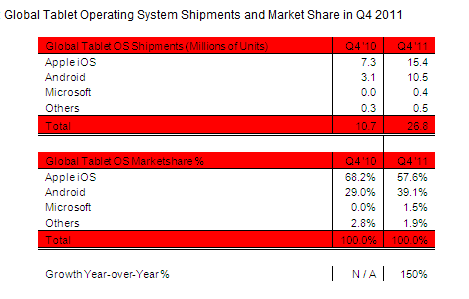
\includegraphics{images/QuarterlySales.png}
	\caption{Shipments refer to sell-in. Numbers are rounded. The definition of tablet does not include e-book readers.\cite{strategyanalytics}}
	\label{fig:QuarterlySales}
\end{figure}



Android is an open-source platform developed for mobile devices. The Android Open Source Project(AOSP) is maintained and further developed by the Open Handset Alliance(OHA), which is led by Google \cite{androidPhilosophy}. The companies from the OHA contributes to the project, these contributions are often made in form of engineering resources.

Android has a large community, spread over various websites, with different areas of expertise. This provides developers of android applications, with a community where they can find help with their nich� \cite{androidCommunity}.
Google, which is head of the android development, also has a website for teaching application developers how to program for the android platform \cite{androidDevelopers}. On Google�s website they also provide various tutorials, so one can easily get started developing for the android platform.

In this project we have been provided with several Samsung Galaxy Tablets 10.1 
\cite{tablet}. The firmware on the tablets is version 3.2\\

NOTE: Stod der ikke noget andet her? Jeg kan ikke finde det mere.

\section{Workform}
		
\chapter{Development methods}
 %\section{Theory}
%	\begin{comment}
One of the goals for this semester is to show that we have knowledge in choosing and implementing different development methods, and apply the method that we find most suited for our project. In order to do this it is necessary to know the different methods, before choosing the best suited. 

Development methods can be put into two categories: Traditional and Agile.

Traditional methods emphasizes analysis and documentation. The structure of a traditional method is therefore often split into phases, for instance the analysis phase or the implementation phase. Once a phase is done you move to the next phase. An example of this is the waterfall method. %TODO [put some example]

Agile methods utilizes an iterative development style, where the focus is on getting a part of the system to work, and then as more iterations are completed, you add to the system until the system is ready to be released. An example of an agile development method
is Scrum. %TODO [put some example]

Both approaches have strengths and weaknesses. The traditional method features lots of documentation and analysis. It also creates a great overview of the whole system, and thus it is easier to estimate how long time it will take before the system is ready to ship. This makes traditional methods well suited for large projects. The agile method on the other hand implements the iteration driven approach. One of the great features of this approach is that you can correct errors and include things you might have forgotten relatively easy, because you just do it in the next iteration. 

One of the big drawbacks of the traditional method is that you cannot just go back a step, if you realize you have forgotten something or made an error. This is very costly because you have to do lots of steps over again. Another big issue with the traditional method is that the customers of the system might not always know what they want or need at the start of the development, but this is where you do all the analysis. The Agile method excels at this as you can present to your customers your current build and receive feedback that you might not have considered. 

The development method that we find best suited for our project is an agile method. This is because in this semester we are working together with educators from institutions working with children with ASD. They will have requirements for our system so it is important that we are taking them into the project. It is also important that we choose a development method that have tools for managing bigger project groups as we are working as part of a bigger team to develop a system.
\end{comment}

In \autoref{sec:devmeth} we decided on using Scrum of Scrums in the multi project.
This does not require us to use Scrum in the project group.
We have considered the following agile development methods:

\begin{itemize}
\item Scrum
\item XP
\end{itemize} 

In short Scrum is a method that emphasizes a self-directed and self-organizing team, each iteration is client driven meaning that the clients provides the requirements and features will be prioritized according to the clients needs\cite{larman}.

XP emphasizes programming and testing. This means that there are very little documentation of the system other than the code. A simple design is preferred and the code is refactored with high frequency. This method requires high discipline since most planning is done orally\cite{larman}.

    In our project it was required that all groups used the same development method to keep things simple. This means that the chosen development method may not be perfectly suited for every group, so while we have chosen the Scrum method we have also made some adjustments to fit it smoother for our group.

The key points of the adjustments are as follow

\begin{itemize}
\item The daily scrum meeting
\item The customer involvement
\item The sprint length
\item Incorporating key elements from Xp method
\end{itemize}

We, in our group, have not utilized the daily scrum meeting that is very typical and defining for the scrum method. The reason for this is that we are already sitting together in the same room. We also know each other well because we have worked together in earlier projects. If we felt like we needed to know anything about the other team members progress we could just ask. We simply did not feel the need to waste time every morning by stating the obvious. We see the daily scrum meeting as a tool for communication. We agree that communication is important to make a great product but we have used alternative ways to communicate.

Customer involvement have been a big focus in the multi project. However our group has been in a different situation than the others because our product has been the server which has little to no interest for the customers. Our biggest requirement providers has been the other groups. This has meant that we have not had a release after each sprint that was shown to the customer for feedback. This was only done once and only for the web interface. As mentioned in section [] a usability test was carried out to get a little more feedback from the customers. 

The sprint length has been modified because the ``number of days'' interval would be misleading because we have some days with lectures and others without. Instead we have define the term ``half days'' which covers either from 8.00 to 12.00 or from 12.00 to 16.00. This interval makes it possible to use days, with lectures covering up half the day, as working days. The sprint length has been dynamic and has been decided at each sprint start. A typical sprint length could be 14 half days which means the next 10 half days to occur. This could be a week without any lectures, or two weeks with lectures. 

There is a specific element associated with the Xp method that we felt the need to incorporate into Scrum, being the pair programming. We have incorporated this element because we find it well suited for programming while leaning. Because we had to learn a new programming language, Java servlet, that none of us had ealier experience in, pair programming helped us a lot in the beginning to quickly catch on.
  \section{Project Backlog}
    \label{sect:pback}
    \input{chapters/proBacklog.tex}

\chapter{Savannah} %TODO temp title
  \section{Requirements} %Martin
	\subsubsection{Initial Requirement gathering}
Requirement gathering was done in the multi project group in the very early stages of the project, but has also been updated as we have been progressing and showing our work to our customers.
In the initial stages we did semi-structured interviews of our customers, where the primary focus was understanding our target group and exploring any tools they currently have access to.
As mentioned the interviews were conducted in a semi-structured manner, we had a few questions%which..are missing?!?
but tried to let the interview run as an informal conversation where the customers could present their own ideas and visions of the project.

From these interviews we created an initial list of requirements for the multi project.
three interviews were done, with Mette and Christina from (ehhh) , Drazenko from (ehh), and Tove from Tale Instituttet(the speech center).
From the individual interviews we gathered a list of their individual ideas and visions and made a requirements list which groups later could refer back to.

\begin{itemize}
 \item Mette And Christina 
  \subitem Customizable software
  \subitem Ease of use, compared to current physical tools
  \subitem Emphasize visual stimuli
  \subitem Continuous stimuli 
 \item Drazenko
  \subitem Customizable software
  \subitem Visual abstract concept
  \subitem Emphasize visual stimuli
  \subitem Unambiguous
  \subitem Consistency/Structure
 \item Tove 
  \subitem Customizable software
  \subitem Engaging/Entertaining software
  \subitem Authentic/proper feedback or behavior
\end{itemize}

From the list of requirements of the individual customers, we identified the requirements which were common for all of them, and made a list of requirements which
should be common for all groups in the multi project.

\begin{itemize}
 \item Customizable software
  \subitem Some way to distinguish unique users on the same tablet is required, since people with autism have very different needs and have very different perceptions of the world.
  \subitem Customization should trump feature bloat.
 \item Emphasize visual stimuli
  \subitem Autistic people are visually over stimulated.
 \item Authentic/proper feedback or behavior.
\end{itemize}

These are all requirements set by our customers, however, since this system is dealing with potentially sensitive personal data, it is 
also a requirement that before it can be deployed in a real world situation, that all transmissions are done via a secure connection. %incomplete 
  \section{Database}
  	%databaseintro.tex
    \subsection{Design}
    	%datadasedesign.tex
The database is designed in MySQL 5.1.61, and resembles the local database created by the ``Admin-group'' very closely -- the only difference is, that the Savanah database has two extra fields in the ``AuthUsers'' table: username and password. The reason for this is, that while all apps running on the android platform uses QR-codes for user authentication, this is not a fitting choice for the webinterface; it would be more complicated to scan the QR-code form a webcam to login, than to simply use a username and password combination.

\subsubsection{Requirements}
The requirements for the database has been provided by the app groups, and are as follows:

\begin{itemize}
	\item All users must be able to login with a QR-code
	\item Each department must also be able to login
	\item All users must be linked to at least one department
	\item All guardians must be able to be linked to at least one child.
	\item All parents must be able to be linked to at least one child.
	\item All users must be able to have access all the apps
	\item All users must be able to access their own pictures, and all public pictures
	\item All departments must be able to access all public pictures
	\item All pictures needs to be able to be linked to different tags
	\item Pictures must be able to be linked with audio and vice versa
	\item A department must be able to have a subdepartment\footnote{Example: ``Birken'' has two departments, at two different addresses, both these subdepartments needs to be linked with ``Birken'' as a superdepartment}
\end{itemize}

\subsubsection*{Diagram}
A database diagram has been made to get a overview of the different tables and their relations. This diagram is designed in DIA, which is a GTK+ based diagram creation program\cite{Dia}, and can be seen in \autoref{fig:DiaDesign}.

\begin{figure}[htbp]
	\centering
		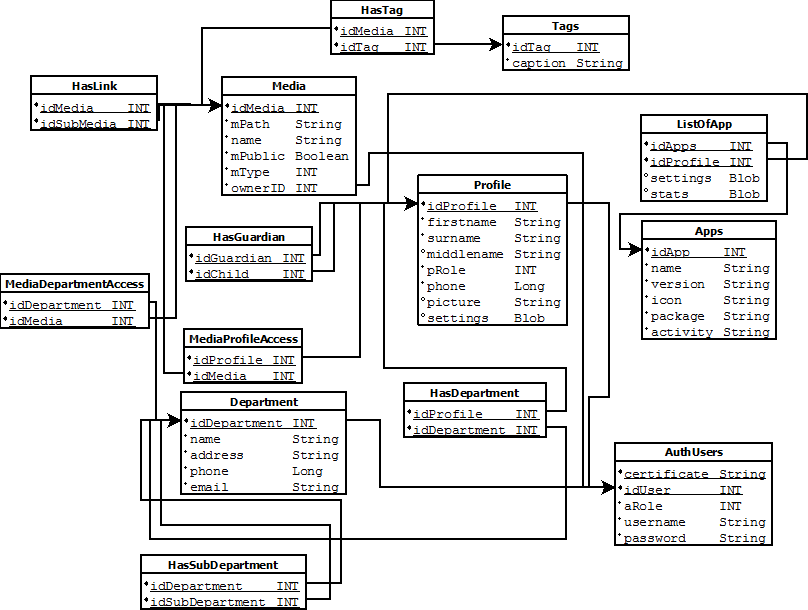
\includegraphics[width=1.00\textwidth]{images/DiaDesign.png}
	\caption{Dia diagram of the database}
	\label{fig:DiaDesign}
\end{figure}

Although the diagram in \autoref{fig:DiaDesign} does not meet the standard of database diagrams, it does provide a good view of the different tables, and the relations: Foreign keys points to where the value is fetched form. This crude diagram shows that be having the ``idUser'' from the ``AuthUsers'' one is able to access all other information for that specific user.

\subsubsection*{Rules}
\label{databaseRules}
To provide the security needed in the system, a few rules need to apply for the databse:
\begin{itemize}
	\item The ``Profile''$\rightarrow$''AuthUsers'' relation must be one-to-one, as one user form the ``AuthUsers'' can only have one profile in the system
	\item The ``Department''$\rightarrow$''AuthUsers'' relation must be one-to-one, as one department form the ``AuthUsers'' can only be one department in the system
	\item The ``idUser'' in ``AuthUsers'' must be unique.
	\item The ``username'' in ``AuthUsers'' must be unique
	\item It must be possible to distinguish between users and departments in the ``AuthUsers'' table
	\item It must be possible to distinguish between children, parents and guardians in the ``Profile'' table
\end{itemize}

These rules will be applied in a mix between SQL script and software level in \textbf{REF TIL SECTION}
    \subsection{Implementation}
    	%databaseimpl.tex
The implementation of the MySQL database is done in MySQL Workbench 5.2.40.

Due to the dependencies of the various tables, the order of how they need to be created is quite strict, see \autoref{MySQLcode}. 
To make sure the \code{username} and \code{userID} attributes follows the previously stated constraints, they have been made \code{UNIQUE NOT NULL} and \code{userID} furthermore has \code{AUTO_INCREMENT} as seen in \autoref{createAuthUsers}. 
This makes sure there can be no one with the same user-name or user ID, and furthermore \code{userID} will automatically increase when new data is inserted. 
This also guarantees a one-to-one relation between both \code{Profile} and \code{AuthUsers}, as well as \code{Departments} and \code{AuthUsers}. 

To distinguish departments and profiles a attribute called \code{aRole} is used. 
This is an integer and will hold a number, which will be used at software level. The same applies for \code{Profile}'s attribute \code{pRole}, see \autoref{createProfile}.

The MySQL Workbench provides the functionality to create an ER diagram from an existing database, this diagram is shown in \autoref{fig:workbenchRight}. The diagram is not completely as MySQL workbench creates it, the real is shown in the appendix \autoref{errDiagram}. But this is a error in the software, as seen in \autoref{fig:workbenchWrong}, the tool generates the \code{Profiles}$\rightarrow$\code{AuthUsers} as a one-to-many relation. However, this is not possible since the \code{idUser} attribute in \code{AuthUsers} is unique, as seen in \autoref{createAuthUsers}, the same goes for both \code{Departments} and \code{Medias}.

\begin{figure}
	\centering
		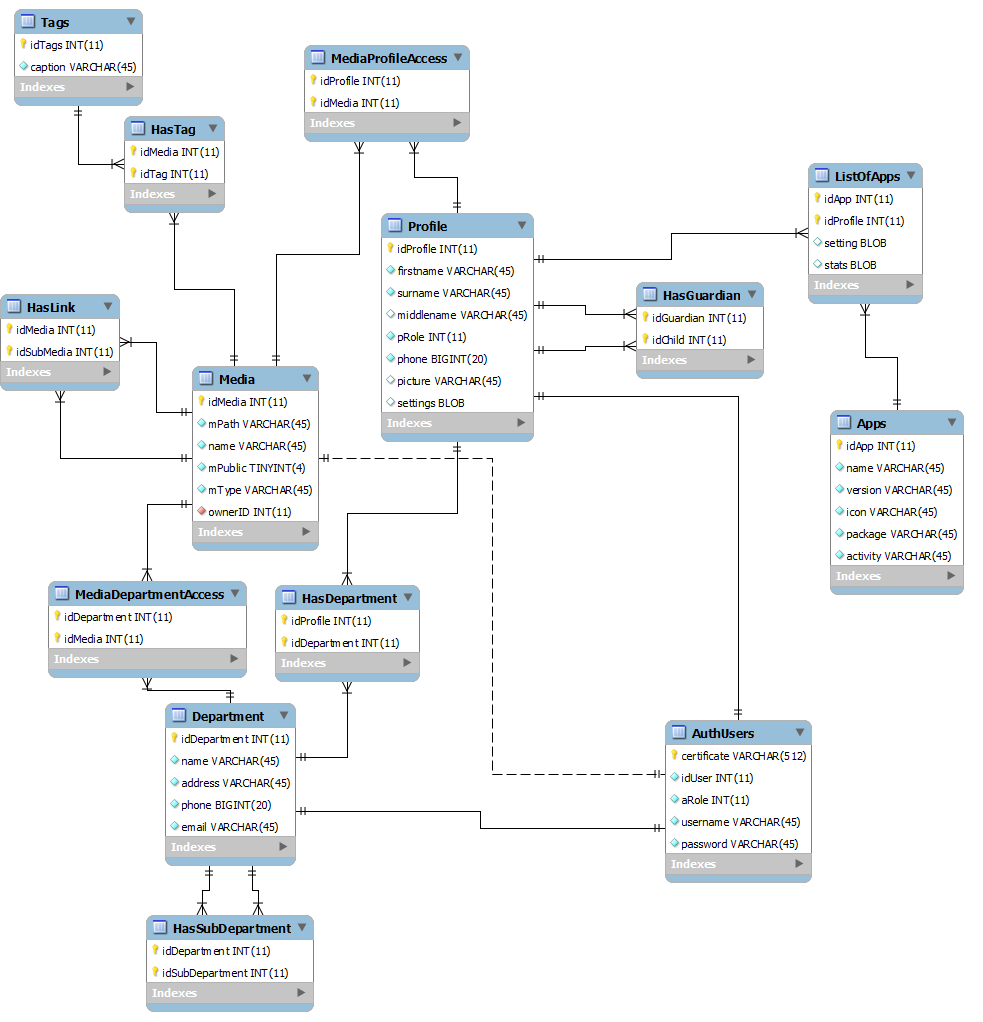
\includegraphics[width=1.00\textwidth]{images/workbenchRight.png}
	\caption{The ER diagram}
	\label{fig:workbenchRight}
\end{figure}

To make the deletion of data easy, many of the attributes in the tables has the constraint \code{ON DELETE CASCADE}. This can be dangerous, as side-effects can result in unintended data being deleted. To avoid this, the software level implementation needs to warn the user when deleting data. Furthermore an analysis has been made to argue which attributes can have this constraint. The following tables and attributes have the cascade constraint: 
\begin{verbatim}
``Profiles''.''idProfile'', 
``ListOfApps''.''idProfile'', 
``HasDepartment''.''idProfile'', 
``HasGuardian''.''idGuardian'', 
``HasGuardian''.''idChild'', 
``Media''.''OwnerID'', 
``HasTag''.''idMedia'', 
``HasLink''.''idMedia'', 
``HasLink''.''idSubMedia'',
''MediaProfileAccess''.''idProfile''.
\end{verbatim}

\subsubsection*{Use case}
 A use case of the constraint is:
\begin{quotation}
``A user ``Jesper'' wishes to delete his entire profile''
\end{quotation}
What will happen is:
\begin{enumerate}
	\item A deletion of the ``userID'' in ``AuthUsers'' is executed
	\item The relation between ``AuthUsers'' and ``Profiles'' will delete the profile
	\item The relation between ``Profiles'' and ``HasGuardian'' will delete all fields where the ``userID'' is either ``idGuardian'' or ``idChild''
	\item The relation between ``AuthUsers'' and ``Media'' will delete all fields where ``idUser'' is the owner
	\item The relation between ``Media'' and ``HasTag'' will delete all fields where ``HasTags''.``idMedia'' equals ``idMedia''
	\item The relation between ``Media'' and ``HasLink'' will delete all fields where ``HasLink''.''idMedia'' or ``HasLink''.''idSubMedia'' equals ``idMedia''
\end{enumerate}


    \subsection{Test}

  \section{Web Interface}
   \label{sect:webInterface}
     \subsection{Programming language}
      %programminglanguage.tex
To be able to provide the desired functionality form the web interface, the web pages must be dynamic and able to interact with the database. There are several different programming languages to choose from. Some of the most common are ASP.net, PHP and Java servlets. Due to the fact that ASP.net is not open source \cite{aspTerms}, and the project is, this is not a feasible choice. This section will do a deeper analysis of PHP and Java servlets, to argue for the best choice of programming language.

\subsection*{PHP}
PHP originally emerged in 1994 when creator Rasmus Lerdorf wrote a simple set of Common Gateway Interfaces (CGI) \textbf{Dette skal forklares} to track visits on his online resume, and decided to name it ``Personal Home Page Tools'' (PHP Tools). As more functionality was desired, he rewrote PHP Tools to fit his demands, and in mid 1995 he released the source code to the public.
\\In 1997 version 3.0 of PHP was released, and the name changed form ``Personal Home Page Tools'' to the recursive acronym ``PHP: Hypertext Preprocessor'' as which it is known today. This is the first version that colsely resembles PHP as it exists today \cite{phpHistory}.


\subsubsection*{Key functionality}

\noindent The following list is a segment of functionality found in PHP 5.4.3. This is based on \cite{phpFunctionality}.

\begin{description}
	\item[Operating system] PHP is supported by all major operating systems, including Linux, many UNIX variants, Microsoft Windows, MAC OSX etc.
	\item[Output] PHP provides the functionality to output not only HTML, but also images, PDF files and Flash movies, all generated on the fly
	\item[Databases] PHP supports a wide range of different databases, including but no limited to MySQL, SQLite and PostgresSQL. The entire list of supported databases can be found at \url{http://www.php.net/manual/en/refs.database.php}. 
	\item[Protocols] PHP can use other service protocols than HTTP, and it is possible to open raw network sockets.
\end{description}


\subsubsection*{Requirements}

\noindent To be able to run PHP on a web server, this needs to support PHP. \href{http://www.php.net/manual/en/tutorial.requirements.php}{Php.net} recommends using Apache web server, and and for database control MySQL \cite{phpReq}.

\subsection*{Java Servlets}
The first version of Java servlets was created by Sun Microsystems in mid 1997, and in December 2009 version 3.0 was released\cite{servletHistory}. It was developed to use the advantages of Java to solve the problems of performance, scalability and security in CGI\cite{servletHistory2}.

\subsubsection*{Key functionality}

\noindent The following list is a segment of functionality found in servlets. This is based on \cite{servletFunctionality}.

\begin{description}
	\item[Portability] Because servlets are written in Java, they are platform independent.
	\item[Power] Servlets can use the full functionality of core Java APIs; this includes URL access, multithreating, image manipulation, database connectivity etc.
	\item[Efficiency] When a servlet is loaded, in remains in the servers memory as a single object instance, this makes it able to handle requests almost immediately.
	\item[Safety] Due to servlets being written in Java, they inherit the strong type safety.
\end{description}

\subsubsection*{Requirements}

\noindent To be able to run servlets on a web server, this needs to support Java servlet. Apache has made a service to allow the execution of servlets, called \href{http://tomcat.apache.org/}{Tomcat}.


\subsection*{Comparison between PHP and servlets}
When comparing PHP and servlets, the focus is put on efficiency and number of active sessions in both languages, as this will be the main requiremtns for the web interface. The following is based on \cite{servletVsPHP} - a research paper by ``IBM Tokyo Research Laboratory''.

\subsubsection*{Efficiency}
The web interface must be able to run fast and smooth, even on high load. A pure benchmark test is found in \autoref{fig:phpVsServlet}. The test calculates a quicksort which sorts 100 integers, A Levenshtein alogithm to measure the similarity between two strings of 56
characters and a Fibonacci execution which calculates the 15th values, with two random starting values. The setup is:

\begin{quotation}
We compared the total run time of
executing each test 10,000 times with each engine. We also executed each benchmark
an additional 10,000 times as a warm-up, before the measured test. This prevents
Java just-in-time compilation overhead from impacting the score in the Java tests.
We ran the experiment on an Intel Pentium 4 CPU at 3.40 GHz with 3GB RAM
Memory, with the Linux 2.6.17 kernel. \cite[p. 167]{servletVsPHP}
\end{quotation}

\begin{figure}[htbp]
	\centering
		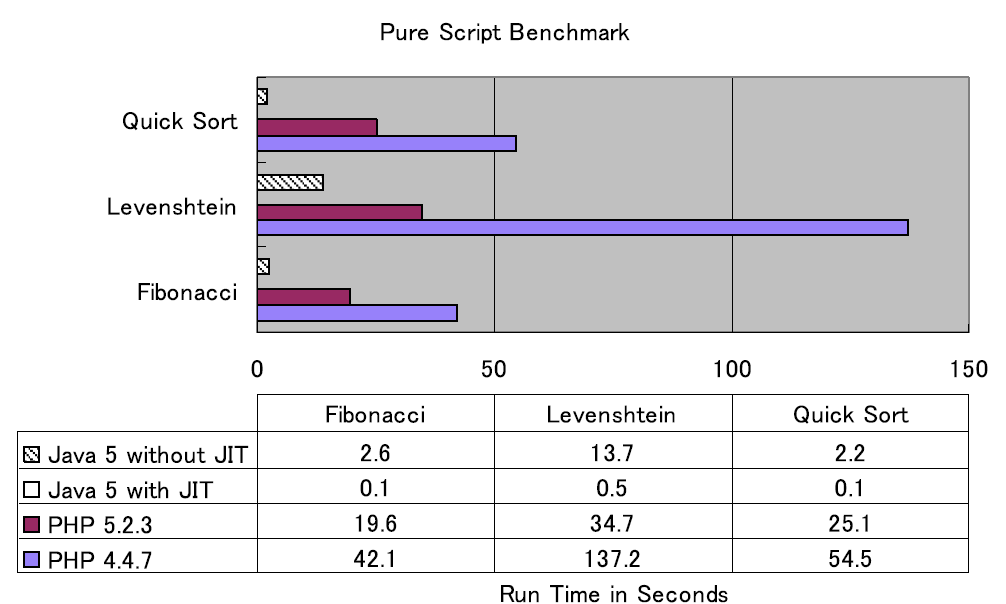
\includegraphics[width=1.00\textwidth]{images/phpVsServlet.png}
	\caption{A pure script benchmark calculating the average time of 1000 \cite{servletVsPHP}}
	\label{fig:phpVsServlet}
\end{figure}

As seen from \autoref{fig:phpVsServlet} servlets are in all test faster, both with and without the Just In Time (JIT) compilation.

\subsubsection*{Sessions}
The web interface must be able to handle many active sessions at the same time. A test of this found in \cite[p. 173]{servletVsPHP}, is shown in \autoref{fig:phpVsServlets2}.

\begin{quotation}
[The figure]... shows the maximum performance for each configuration and scenario, as
determined by the maximum number of simultaneous sessions (e.g., users) which can
be supported with acceptable Quality Of Service as defined by SPEC \cite[p. 173]{servletVsPHP}.
\end{quotation}

\begin{figure}[htbp]
	\centering
		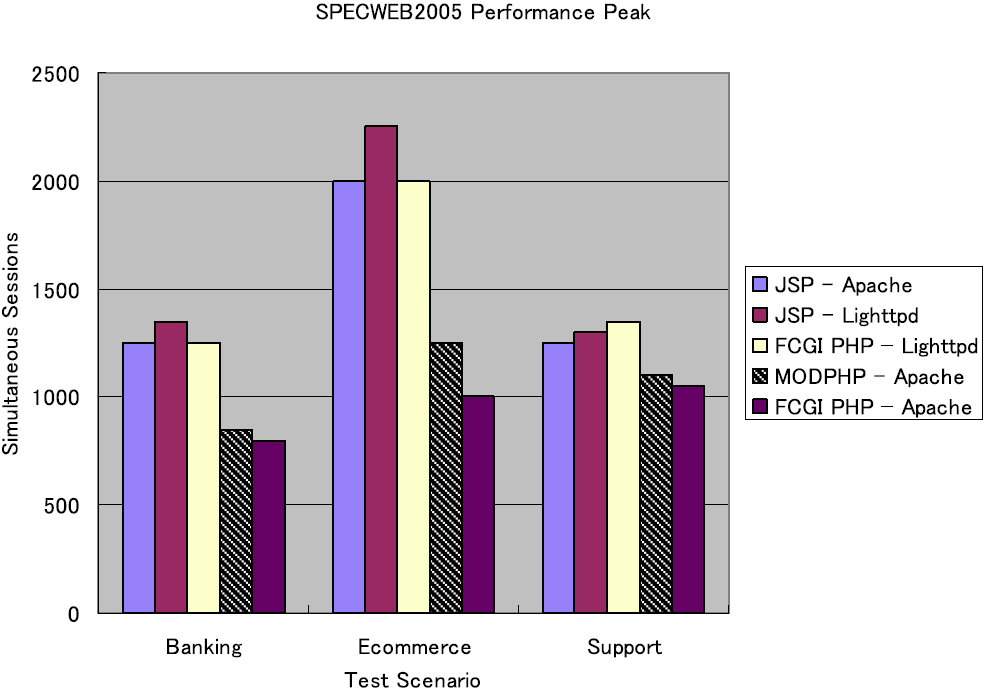
\includegraphics[width=1.00\textwidth]{images/phpVsServlets2.png}
	\caption{TROLOLOLO}
	\label{fig:phpVsServlets2}
\end{figure}

\autoref{fig:phpVsServlets2} shows that in 2 out of 3 test cases JSP is able to handle more active users than PHP.

Even though the servlets genually is more powerfull than PHP, this only comes to show, when the servler load is high (around 750 active sessions at the same time). Eventhough the efficiency of JSP is better than PHP \cite{servletVsPHP} sums up the descussion quite well:

\begin{quotation}
When implementing a web server system which will never experience high load, or in
which performance, throughput, and reliability under high load is not an issue, then
the use of any of the analyzed languages or web servers will achieve similar
performance results. If outstanding performance and throughput is the primary goal,
then the use of JSP over PHP is advisable. However, if a 5-10\% difference in
throughput and performance is acceptable, then the implementer of a web system can
achieve similar results using either PHP or JSP. In which case, other requirements
such as developer language familiarity and programming efficiency, maintainability,
security, reliability, middleware compatibility, etc. would be the deciding factors \cite[p. 181]{servletVsPHP}.
\end{quotation}

We have chosen to implement the web interface in servlets, due to the facts that we have a lot of experience in Java already and the Andoid apps are developed in Java, so choosing this seems fitting.
     \subsection{Implementation}
     	%webimpl.tex
This section describs the work of implementing the web interface in Servlets.

\subsubsection{Mockups}
To get startet at series of mockups was created, to get an idea of the geneal look and feel of the website. An example of this is shown in \autoref{fig:mockSelectProfile}, the rest can be found in \autoref{app:Mock}.

\begin{figure}[htbp]
	\centering
		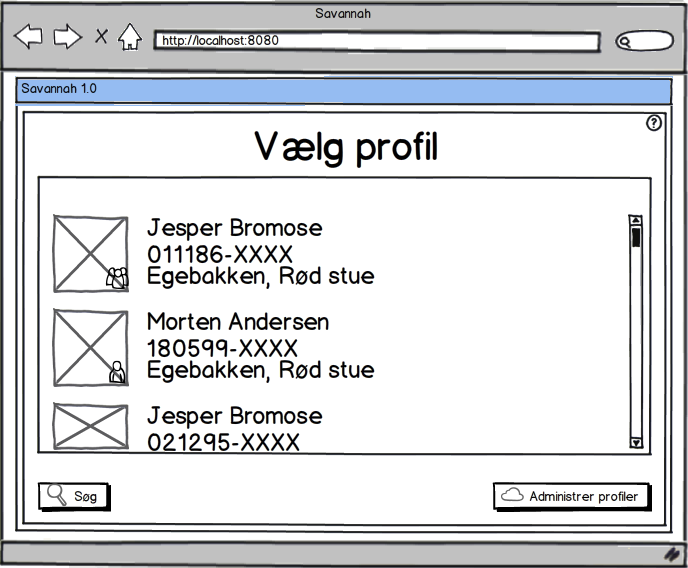
\includegraphics[width=1.00\textwidth]{images/mockSelectProfile.png}
	\caption{A mockup of profile selection}
	\label{fig:mockSelectProfile}
\end{figure}

\subsubsection{Programming languages}
The web interface uses four different languages: Servlets, HTML, JavaScript, and Cascading Style Sheets (CSS). The Servlets are used responisble for database access, and generation of both the HTML code and JavaScript, and the CSS is used for for the graphic on each page. The HTML is used for making the elements on the webpages, and the JavaScript is sued to add some dynamic to a generated HTML side.

\subsubsection{Structure}
The structure of each Servlets page is seen in \autoref{fig:webStruct}
\begin{figure}
	\centering
		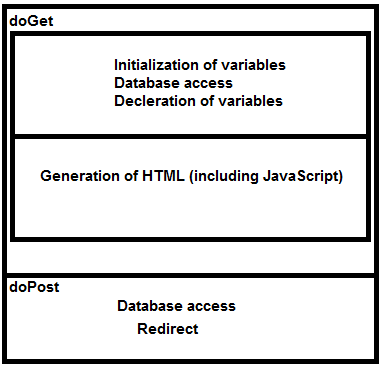
\includegraphics{images/webStruct.png}
	\caption{General structure of Servlets}
	\label{fig:webStruct}
\end{figure}

When a webpage is first loaded, it access the \code{doGet} code, and executes the code within. After this there are three scenarios:
\begin{description}
	\item[Scenario 1] The user click a link, and is sent to a new page.
	\item[Scenario 2] The user submits a \code{form} with \code{doGet} method. 
	\item[Scenario 3] The user submits a \code{form} with \code{doPost} method.
\end{description}

In scenario 1, the current pages do not do anything else but send the user to the new page, which executes the code in its \code{doGet} code. In scenario 2 the \code{form} structure dictates what happens: It can either redirect to itself, and execute the \code{doGet} method again \autoref{code:getRedirectSelf}, or redirect to a new page and execute the \code{doGet} method on that, see \autoref{code:getRedirectNew}.

\begin{lstlisting}[language=Java,label=code:getRedirectSelf,caption=A form which redirect to its own get method]
	@WebServlet("/DeleteTags")
	
	/**
	 * @see HttpServlet#doGet(HttpServletRequest request, HttpServletResponse response)
	 */
	protected void doGet(HttpServletRequest request, HttpServletResponse response) throws ServletException, IOException {
	
	out.println("<center><form method='GET' name='formName' action='DeleteTags'>");
	}
\end{lstlisting}

\begin{lstlisting}[language=Java,label=code:getRedirectNew,caption=A form which redirect to its own get method]
	@WebServlet("/DeleteTags")
	
	/**
	 * @see HttpServlet#doGet(HttpServletRequest request, HttpServletResponse response)
	 */
	protected void doGet(HttpServletRequest request, HttpServletResponse response) throws ServletException, IOException {
	
	out.println("<center><form method='GET' name='formName' action='NewPage'>");
	}
\end{lstlisting}

Secnario 3, has almost the same code as \autoref{code:getRedirectSelf} and \autoref{code:getRedirectNew}, with the excpetion that the \code{method='POST'}.

In generalt the \code{form} is build as \code{<form method='POST/GET' name='NameOfForm' action='WhichPageToExecuteCodeFrom>}.

\subsubsection{Database access}
The read data from the database is handled by Java code in each of the Servlets, the code is shown in \autoref{readDatabase}. To update attributes in the database, the \code{stmt.executeQuery} is used, with the appropriate SQL script.  To delete data, instead of \code{stmt.executeQuery} a \code{PreparedStatement} is created, this is executed with by calling \code{int i = ps.executeUpdate();} which will give either a OK code (0) or and error code. 

\begin{lstlisting}[language=Java,label=code:readDatabase,caption=Code to read data from the database]
public void readData()
{
String dataVar;
Connection con = null;
Statement stmt = null;
ResultSet rs = null;
try {
   Class.forName("com.mysql.jdbc.Driver"); //Use this driver to access the database
   con = DriverManager.getConnection("jdbc:mysql://DatabaseAddress", "Username", "Password"); //Instansiate the connection
   stmt = con.createStatement(); //Instansiate stmt
   rs = stmt.executeQuery("SQL query"); //Executes the SQL query and get the result store in RS
   //As long rs contains data, read it!
   while (rs.next()) { 
      String name = rs.GetString("Name"); //Get a string attribute
      int number = rs.GetString("Number"); //Get a int attribute
}
//Error handeling
catch (SQLException e) 
{		
   throw new ServletException("Servlet Could not display records.", e);
} 
catch (ClassNotFoundException e) 
{			
   throw new ServletException("JDBC Driver not found.", e);
}
//Make sure the connection is closed, no matter what 
finally {
   try {
      if (rs != null) {
         rs.close();
         rs = null;
      }
      if (stmt != null) {
         stmt.close();
         stmt = null;
      }
      if (con != null) {
         con.close();
         con = null;
      }
   } 
catch (SQLException e) 
{			
}
}

\end{lstlisting}

\subsubsection{Generation of the web page}
The generation of the web page, is done within the servlet, using a \code{PrintWriter}. This is instansiated by cy calling \code{PrintWriter out = response.getWriter();}, and used to write the HTML code by calling \code{out.println("HtmlCode");} which will generate a web page, with only THAT code visible. \code{out} can furthermore be used to write both JavaScript and CSS.

The CSS however is not written within any of the Servlets, instead is i located in a seperate file \verb+/WebContent/CSS/SavannahStyle.css+ and is included in the HTML by \code{ "<link rel='stylesheet' type='text/css' href='CSS/SavannahStyle.css' />"}


\subsubsection{Exchange of data}
When a Servlet submits a form, the data is sent differently depending on the \code{form} method. A \code{GET} method will send the data as a part of the URL thus make it visible for the user, as seen in\autoref{code:URLLINK}, where as the \code{POST} method does not make it visible.

\subsubsection{\code{Form} data}
To access the data from the \code{form}, this needs a name. The name it set by the \code{name} attribute in the \code{input} element. The type of data sent from the \code{form} depends on the type of element.
\begin{description}
	\item[\code{Text},\code{Password} and \code{TextField}] The value of these fields are of the type string, and contains the value entered
	\item[\code{RadioButton}] All \code{RadioButton}s with the same name, sends the value of the selected \code{RadioButton}
	\item[\code{CheckBox}] All \code{CheckBox}es with the same name sends the value of each checked box.
	\item[\code{DropdownBox}] Sends the value of the selected item
	\item[\code{ListBox}] Send the value of all the selected items as a string array
\end{description}

\begin{lstlisting}[language=Java,label=code:URLLINK,caption=URL with visible parameters]
http://www.xoxoxoxox.com/servlet/ServletName?var1=value&var2=value&var3=value
\end{lstlisting}

To be able to retrieve the data sent by the form the \code{request.getParameter()} method is used. An example of this is shown in \autoref{code:getDataInPost}.

\begin{lstlisting}[language=Java,label=code:getDataInPost,caption=How to read parameters]
	@WebServlet("/PseudoClass")
	/**
	 * @see HttpServlet#doPost(HttpServletRequest request, HttpServletResponse response)
	 */
	protected void doPost(HttpServletRequest request, HttpServletResponse response) throws ServletException, IOException {
		String myVar = request.getParameter("FieldName"); //Get single Value
		String[] myVarArray = request.getParameterValues("FieldName") //Get string array
	}
\end{lstlisting}

\subsubsection{Current limitatio}
When uploading a picture, a \code{file} type is used to select the local file on the hard disk. The \code{file} has a security restricting, which makes it impossible to set a default value for the field. This is due to the fact, that if it was possible, it could be used to send a file from the visitor of a web page's hard disk, without the visitor has any knowledge of it\cite{noFile}. Futhermore it was not straight forward to get the path of a selected file, again due to security restrictions, but this turned out to be possible by the use of JavaScript, the code is seen in \autoref{code:myHack}, and adding parameter \code{onChange="readURL(this);"} to the \code{file} field.

\begin{lstlisting}[language=HTML,label=code:myHack,caption=Hack to load file from \code{file} box]
var reader = new FileReader();+
reader.onload = function(e) 
   {
      document.billedet.src  = e.target.result;
   };

function readURL(input)
   {
      if(input.files && input.files[0])
      {
         reader.readAsDataURL(input.files[0]);
      }
      else 
      {
         document.billedet.src = "";
      }
   }
\end{lstlisting}


     \subsection{Test}
		In this section we have described the tests we have made for our web interface. First we present our results from the usability test, then we present the test cases and the results.

\subsubsection{Usability Test}

Our usability test was carried out using the IDA method, described in \autoref{common:sec:usabilitytest}. The results are as shown in \autoref{tab:results}

\begin{table}[H]
	\scriptsize
	\centering
	\begin{tabular}{|p{7cm}|r|l|}
		\hline
		Error & Frequency & Category \\
		\hline
		\hline
		Create a profile was difficult and counter intuitive & 3 & Serious \\ \hline
		The home button was only on some sites and confuses the user & 5 & Serious \\ \hline
		/imagenull would appear for no reason when a user was created & 3 & Cosmetic \\ \hline
		HTTP errors during the test & 5 & Critical \\ \hline
		Access to apps caused confusion, the user could not figure out what it was used for & 5 & Cosmetic \\ \hline
		Choose file was not further specified and caused confusion & 3 & Cosmetic \\ \hline
		GUI size was not filling up the whole screen which some of the test subjects found inconvenient & 2 & Cosmetic \\ \hline
		QR-code page misunderstanding home link & 3 & Cosmetic \\ \hline
		Add guardian to child was counter intuitive & 3 & Critical \\ \hline
		Edit profile made the users believe that they had to change password every time & 2 & Serious \\ \hline
		When logging in on child's profile as guardian the dropdown menu was confusing & 4 & Serious \\ \hline
		The user was confused of what to do after login & 1 & Cosmetic \\ \hline
		Edit/add picture was confusing & 3 & Serious \\ \hline
		The phone number was required but this is not the situation in reality & 5 & Critical \\ \hline
		Missing caption for choosing role causes confusion & 1 & Cosmetic \\ \hline
		The test subject was unsure which tags corresponded to which check-box & 2 & Critical \\ \hline
		Confusing, too many options & 1 & Serious \\ \hline
		The test subject tried to login as one of the predefined users because they thought it was their profile & 2 & Cosmetic \\ \hline
		The user lost the overview & 5 & Serious \\ \hline
		The user was not sure which pictures were public when asked to delete a public picture & 1 & Cosmetic \\ \hline
		When deleting pictures, the tags in brackets caused confusion and the text fields implied that you could write in them which is not the case & 1 & Cosmetic \\ \hline
		The test subject was unsure how to get back from the audio page & 1 & Cosmetic \\
		\hline
	\end{tabular}
	\caption{Results of the usability test}
	\label{tab:results}
\end{table}

In summation: 11 errors were defined as cosmetic, 7 as serious, and 4 as critical. \\

The critical errors were that the page broke down with an error. another critical error was that a phone number was required for a child, while it should be optional.
This is a requirement that has not been implemented, because we have not received the request before the test.
When prompted to add a guardian to a child there was confusion on how to do that.
The reason is mainly because it is not placed in an intuitive place, and the test subjects had to get help from the test monitor.
The last critical error was the tags selection. The problem was that the user did not know, if a checkbox was assigned to the caption above or below. While this seems as a cosmetic or serious problem at worst, while the user was experimenting with the tags, the system crashed for unknown reasons. We have not been able to recreate this crash so we have rated the problem as critical although the system might not crash.

The rest of the problems found in the test was primarily things missing, bad layout, or misplaced functionality.
Missing things include ``back'' or ``home'' options from certain pages or captions that tells the user what certain fields require as input when filling out formulas. Bad layout is the main reason for confusion when using the system, this could be too much information presented to the user at once.
Misplaced functionality includes the placement of the profile list on the main page, which a lot of users thought related to editing and adding profiles -- leading to confusion. 

  \section{serverside} %TODO temp title
    The following section concerns the design and implementation of the server side software for Savannah and the sw6ml language, 
which is an XML language designed for data transfers.
    \subsection{Architechture and Design}
      \label{sect:ssArchAndDesign}
      \subsubsection*{Architecture}
An overall design and architecture was created in the early sprints of the project.
The server side software is different from the rest of the software made in the multi project group, in that the the customers will never actually see it in action, it works perfect if they never notice it is there.
Almost all requirements from our customers concern the user interface and general feel of the apps for the mobile devices. In regards to the server software it is the requirements of the multi project that are of interest,
in particular the oasis group, as their responsibility is to link the rest of the world to us.

The giraf system is designed in such a way that it deploys with two databases: Savannah - our project, a global database for a full deployment unit, and Oasis - or localDB, a local database which exists only
on the mobile devices, which has an almost identical schema to Savannahs database.
Rather than having Oasis query the global database directly, it was decided to implement access to both the databases through a software layer, as shown in \autoref{fig:softwareLayers}.
The pros and cons of this seemingly redundant software layer was considered, see \autoref{table:proconSoftwareLayers}

\begin{figure}[H]
	\centering
		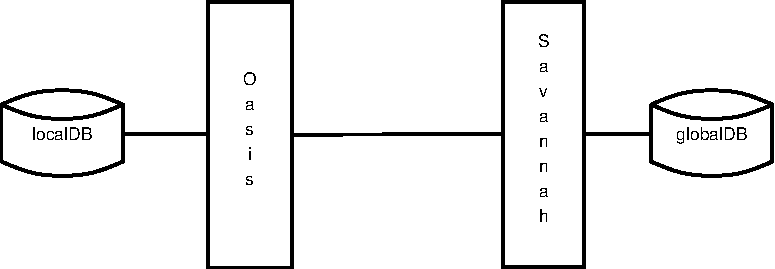
\includegraphics[scale=1]{images/softwareLayers}
	\caption{Software layers}
	\label{fig:softwareLayers}
\end{figure}

\begin{table}[H]
  \begin{center}
    \begin{tabular}{c|c}
    Pros                   &             Cons \\
    \hline
    More flexibilty        & higher complexity\\
    Independent DB updates & Lower performance\\
    \end{tabular}
    \caption{pros and cons of an extra software layer between the databases}
    \label{table:proconSoftwareLayers}
  \end{center}
\end{table}

Having an extra software layer between the databases means we can alter the global and local databases independently of each other. By providing software with methods for extracting specific
details from Savannah, like full profiles, oasis does not have worry about Savannahs internal database schema. The downside of this is that the complexity inevitably will be higher, and performance
will be lower, the performance issue is not critical though, since the perceived performance of the system will be dominated by the bandwidth of the mobile devices. 
The communication between the software layers will be facilited by the sw6ml XML language, presented in \autoref{sw6ml}

Savannah has a three layered internal architecture, show in \autoref{figure:savaArch}.

\begin{figure}[H]
  \centering
    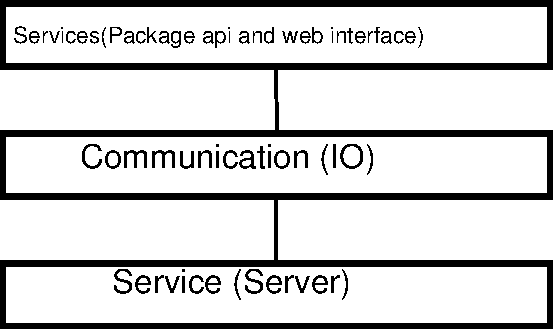
\includegraphics{images/savaArch}
  \caption{Savannahs architecture}
  \label{figure:savaArch}
\end{figure}

A short description of each layers responsibilities follows:

\begin{description}
 \item[Services] The services layers consists of the services that we provide to external users. We have considered two services to include, which are an API for creating transmissions packages	 		that savannah understand, and the web interface discussed in \autoref{sect:webInterface}.
 \item[Communication] The communication layer consists of the IO package of the server side software, which handle retrieval and responding.
 \item[Service] The service layer consists of event handling, query handling and building of sw6ml documents.
\end{description}


\subsubsection*{Design}
The overall server software is designed around a producer-consumer pattern, where Oasis acts as the producer through savannah's IO layer.
Request or commit packages send to savannah will be processed by the \code{IOHandler} which will add an event to the \code{EventQueue}. The consumer is the server itself, which will remove events from the queue and process its content, being it a request or a commit. Using a queue based design was chosen to for sake of simplicity, the project is a part of learning process and building a server with concurrent event handling was down prioritized versus a simpler server, which would allows us to gain experience and still meet the requirements of the study regulations.
 A mock overview of the design of the server can be seen in \autoref{figure:serverMockup}, this diagram represents the general idea and flow of the server and should not be understood as formal technical specification.
\begin{figure}[H]
 \centering
  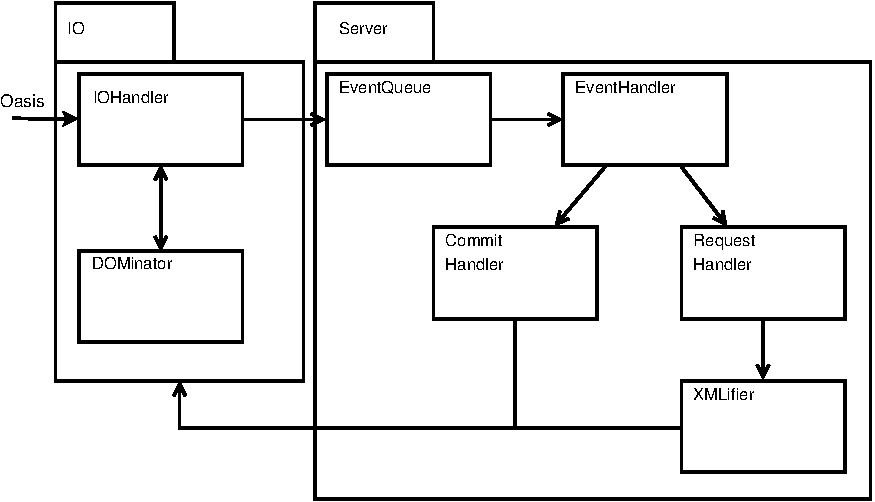
\includegraphics[scale=1]{images/savaIniDesign}
 \caption{Savannnah server Mockup}
 \label{figure:serverMockup}
\end{figure}

      \subsubsection{sw6ml} %Martin
         \label{sw6ml}
	  %Introduction
In order to facilitate consistent data transfer between the global database and localDB, we have designed an XML language which mimics
the schema of the database. We have chosen to use XML as it is a recognized standard, with a wide array of tools available, in particular JDOM\cite{www.jdom.org}.
JDOM is a light weight implementation of SAX and the Data Object Model(DOM) for java, which allows seamless integration of XML, with support for XPath and XSLT.
In \autoref{sw6mlusage} a short usage documentation for sw6ml is provided. sw6ml is defined with XML schema.

\subsubsection{Language Design}

The sw6ml language consists of a number of primary elements which reflect the tables in the database, each of these elements accepts any number of ENTRY elements that tell
the server what action is should do with the incomming data.
in \autoref{code:sw6mlExample01} a short example of legit sw6ml syntax for adding a row to the AuthUsers table and deleting a row with the idUser table attribute equal to 2 is shown.
The \code{<AuthUsers>..content..</AuthUsers>} element identify the table on which we want to make changes, the following \code{<Entry>..content..</Entry>} elements
define what row and what kind of action, through the \code{action="foo"} xml attribute, should be done on the row. 

\begin{figure}[H]
\begin{lstlisting}[label=code:sw6mlExample01,caption=Example of sw6ml syntax]
 <AuthUsers>
    <Entry action="create">
      <certificate type="string">This is a certificate</certificate>
      <idUser type="int">1</idUser>
      <arole type="int">1</arole>
      <username type="string">mette</username>
      <password type="string">obfuscated</password>
    </Entry>
    <Entry action="delete">
      <idUser type="int">2</idUser>
    </Entry>
  </AuthUsers>
\end{lstlisting}
\end{figure}
The \code{action="foo"} xml attribute has four legal types corresponding to the CRUD profile actions, create, read, update, and delete, shown in \autoref{code:sw6mlCrud}.
Contained in the  \code{<Entry action="crud_type`">..content..</Entry>} element is a series of 0 or more elements corresponding to the table schema of, in this case, the AuthUsers table.
It takes zero or more of the table attributes in a row, since not all table attributes are needed for all actions, as an example delete only requires the unique identifier of the table and
updates will only need the unique identifier and the table attribute being updated.
\begin{figure}[H]
\begin{lstlisting}[label=code:sw6mlCrud,caption=sw6ml crud simple type]
 <xs:simpleType name="crud">
  <xs:restriction base="xs:string">
    <xs:enumeration value="create"/>
    <xs:enumeration value="read"/>
    <xs:enumeration value="update"/>
    <xs:enumeration value="delete"/>
  </xs:restriction>
</xs:simpleType>
\end{lstlisting}
\end{figure}

\subsubsection{Documentation}
\label{sw6mlusage}
To use the current version of sw6ml and savannah together it is essential to know the elements required from the different crud types.
while XML schema provides advanced features for dynamic languages, sw6ml int its current version, is a primitive language consisting of simple types and sequences.
this is however all that is needed, with a few assertions on the format server side.

\autoref{code:sw6mlformal} show the formal structure of a sw6ml document.
\begin{Code}
\begin{lstlisting}[label=code:sw6mlformal,caption=root and table elements]
<sw6ml> 
  <table_element_1>
    <Entry action="crud_type">
      <table_element_1_attribute_1/>
	...
      <table_element_1_attribute_n/>
    </Entry>
  </table_element_n>
  ...
  <table_element_n>
    <Entry action="crud_type">
      <table_element_n_attribute_1/>
	...
      <table_element_n_attribute_n/>
    </Entry>
  </table_element>
</sw6ml>
\end{lstlisting}
\end{Code}

following is a short description of the setup of the \code{<Entry>} element for each crud type.

\begin{description}
 \item[create] creates a new row in the database: All attributes from the database schema is required, if no value exists, use null. See \autoref{code:sw6mlExample01} for an example.
 \item[update] Updates a field in a row, Required in this order: Unique identifier of the row, Attribute to be updated. See \autoref{code:sw6mlExample02} for an example.
 \item[delete] Deletes a row in the able: Only the unique identier is required. See \autoref{code:sw6mlExample01} for an example.
 \item[read]   Read is only used in xml which is send back on a request to the server, and thus require no special formatting.
\end{description}

Notice the \code{<row_attribute type="bar">..</..>} xml attribute, legal types are \code{string} or \code{int}, if the data type of the row attribute is a string or any other type requiring apostrophes
in a sql query, use \code{string}, for anything else use \code{int}.

\begin{lstlisting}[label=code:sw6mlExample02,caption="sw6ml Update syntax example]
 <Entry action="update">
   <unique_identifier type="bar">foo</unique_identifier>
   <attribute_to_be_updated type="bar">newValue</attribute_to_be_updated>
 </Entry>
\end{lstlisting}

The sw6ml schema can be found on the project repository together with a valid sw6ml document,
Full path: \url{http://code.google.com/p/sw6-2012/source/browse/random_group_stuff/Group_server/xml/sw6_schema.xsd}
and \url{http://code.google.com/p/sw6-2012/source/browse/random_group_stuff/Group_server/xml/sw6_example.xml} %TODO fix this document before handin;-)


	  
    \subsection{Implementation}
      \subsubsection{Input handling} %Thorbjørn
		When the server starts it will execute a method called \code{listen()} that listens for any connections, see \listref{code:listen}.
Whenever any \code{Socket} connects to the server, the \code{listen()} method will create a new \code{CommunicationThread}.
This thread will then read the information in the \code{Socket}'s \code{InputStream} and depending on the connection type (commit event, request event or ping) it will deal with it appropriately.

\lstinputlisting[label=code:listen,caption=Method: \code{listen()}]{code/IOHandler-listen.txt}

In the following subsections we will explain how the different types of connections are processed by the system.


\subsubsection{Ping}
\label{sec:IOPing}

Diagram ledger: (see \figref{fig:IOLedger})\newline
The uppermost port is used to indicate input and the lowermost port is used to indicate output. The arrows indicate which way the information is forwarded in the system. Any arrows leading to and fro a component, and not from an input or output port, are to be executed first.	\newline
\begin{figure}[H]
	\centering
		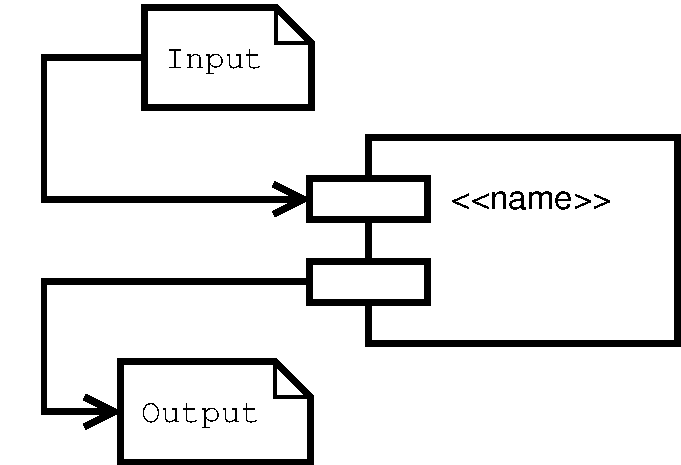
\includegraphics[scale=0.40]{images/ledger} %FIXME epstopdf package fucker, har ændret noget her
	\caption{Ledger for diagrams}
	\label{fig:IOLedger}
\end{figure}

%	The \newlines are to prevent the words from "running" out of the page - don't know why this happens :(
% This has been tested with   \texttt{arg} and \code{arg}
Figure \ref{fig:IOPing} is a model of how a ping is process by the server. The \code{Connection} component sends output, in this case a ping event, to the server. In the server this is received by the \code{IOHandler}, which creates a new \newline \code{CommunicationThread}.
The \code{CommunicationThread} will then use the \newline \code{TransmissionHandler} to determine if the input is of the type commit, request or ping.
In this case the input is of the type ping, and it will just directly respond to the caller (connection).
\begin{figure}[htbp]
	\centering
          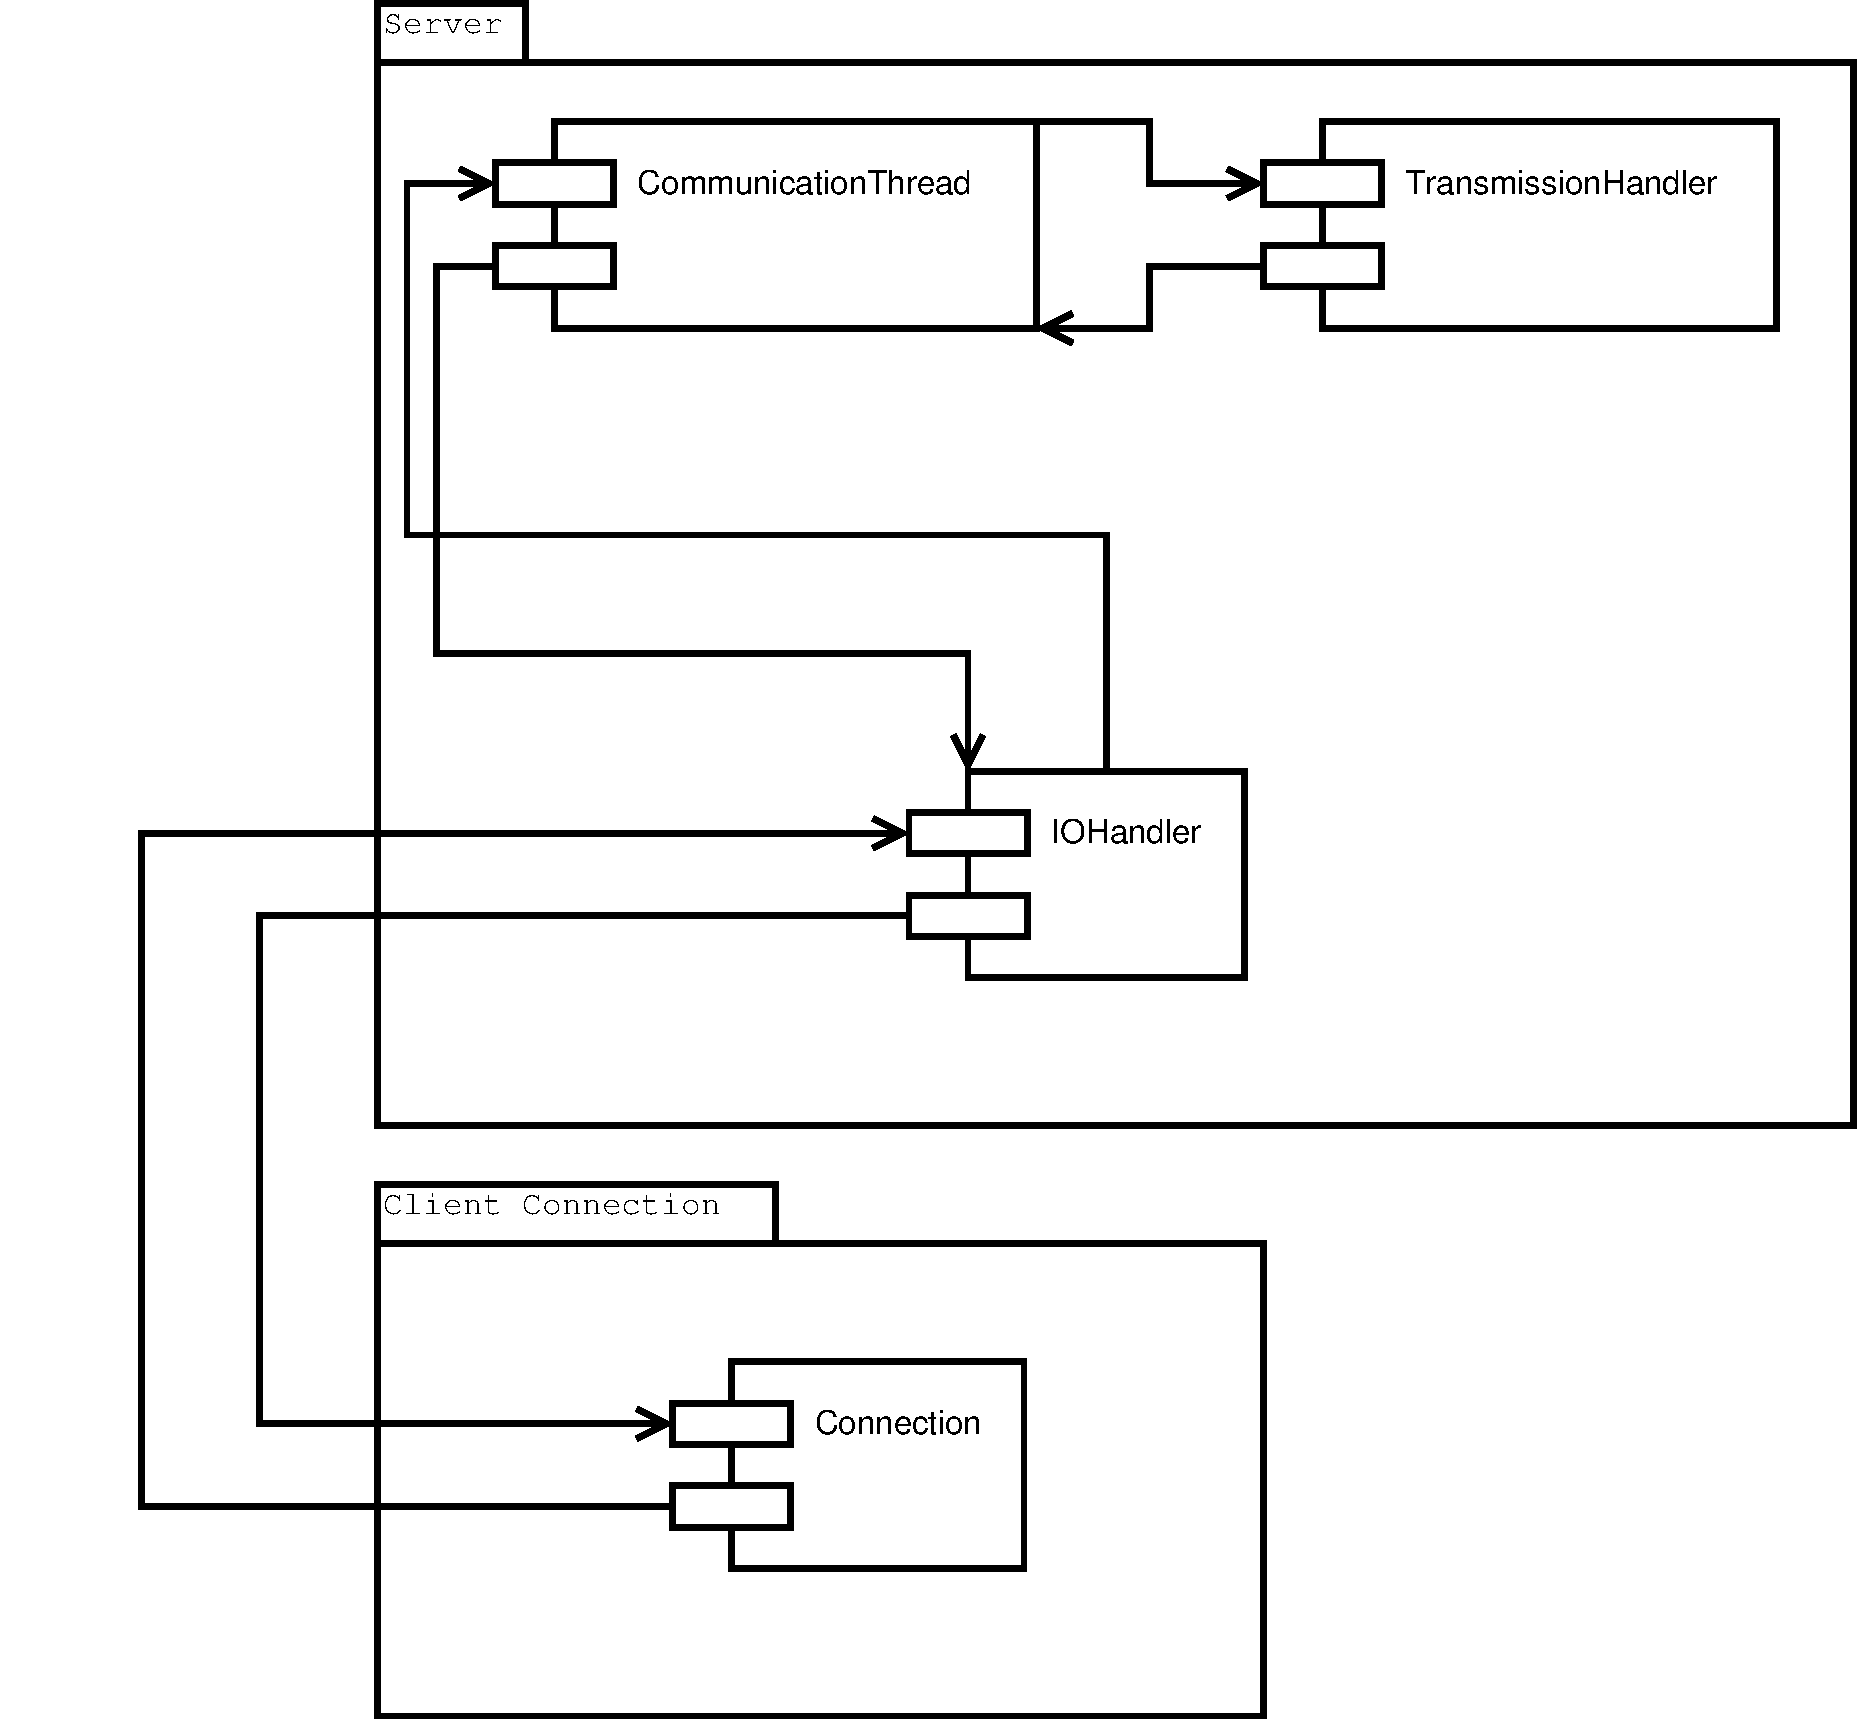
\includegraphics[scale=0.30]{images/ping}%FIXME epstopdf packager fucker, har ændret til at bruge de generede pdf filer direkte
	\caption{A diagram illustrating how a ping is processed.} 
	\label{fig:IOPing}
\end{figure}

%	The \newlines are to prevent the words from "running" out of the page - don't know why this happens :(
% This has been tested with   \texttt{arg} and \code{arg}
The reason for this implementation is that Java only supports two types of sockets: stream based (TCP --- \code{java.net.Socket} and \code{java.net.ServerSocket}) and datagram based ones (UDP --- \code{java.net.DatagramSocket} \newline and \code{java.net.MulticastSocket})\cite{ICMP}\cite{javaNET}. However an implementation of ping would require the use of ICMP(Internet Control Message Protocol) ping, and since this is not possible we have chose to implement a ping at a software level, rather than as a protocol.


\subsubsection{Commit and Request}
\label{sec:IOCR}
For a connection of type commit or request, the procedure is almost the same. However, when the \code{CommunicationThread} has been created and its \code{TransmissionHandler} has determine the type of the connection, it will opposite for the ping, create a new event corresponding to the type and send it to the \code{EventHandler}, see \figref{fig:IOCR}.
First when the \code{EventHandler} is done processing the event, will the server respond to the connector.
To see how the \code{EventHandler} processes the given queries see \secref{QQHandling}.

\begin{figure}[htbp]
	\centering
		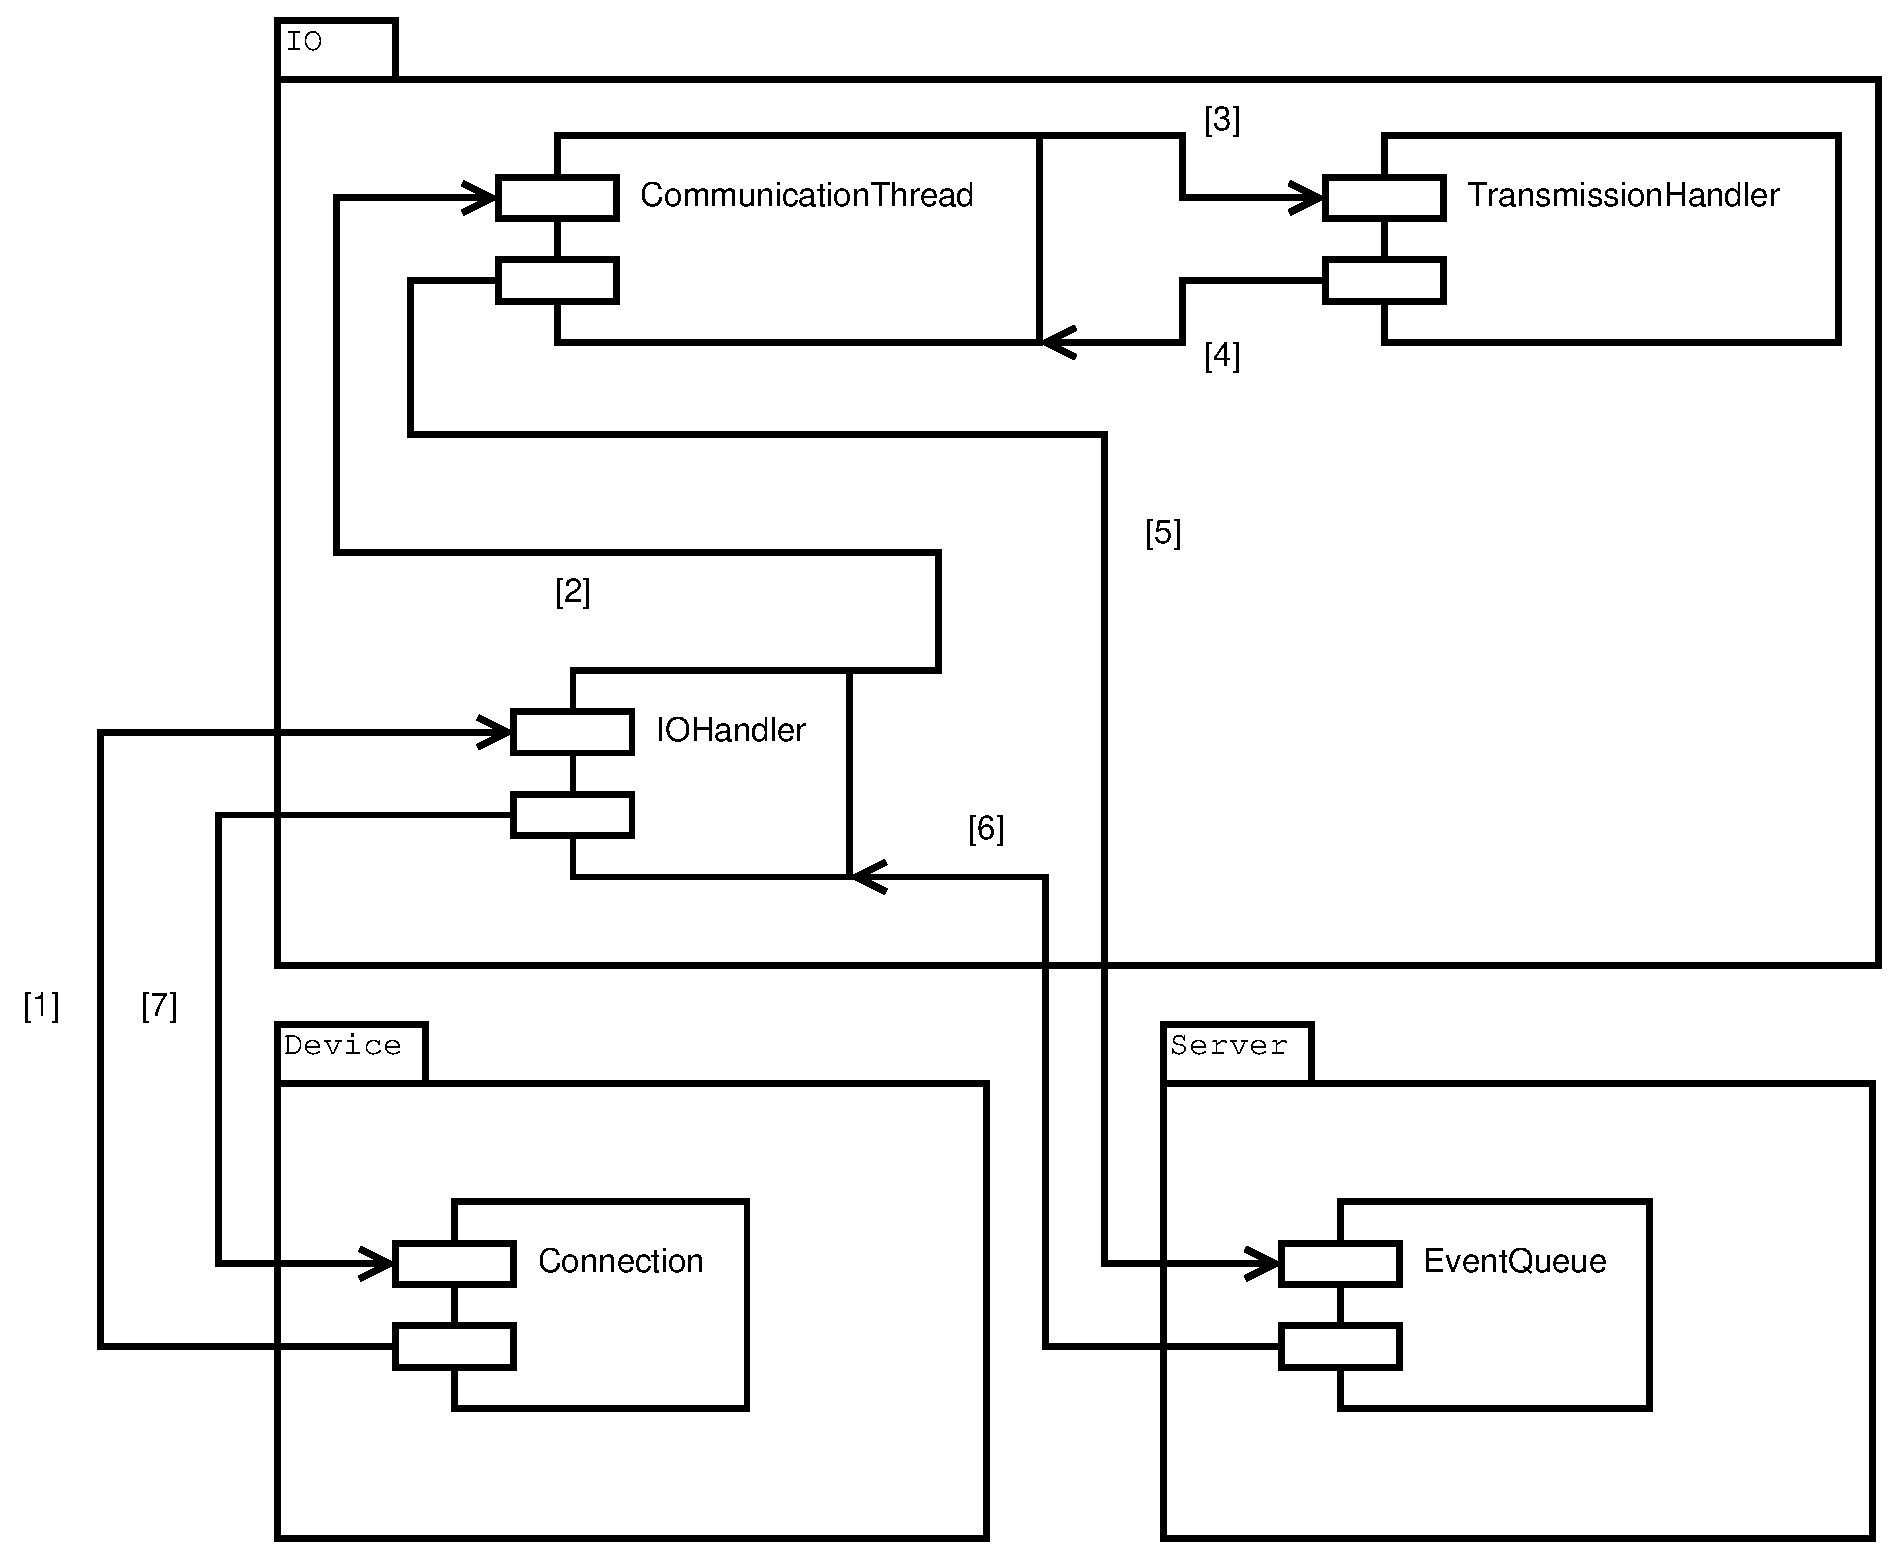
\includegraphics[scale=0.30]{images/requestCommit.eps} %FIXME epstopdf package fucker, men har ikke ændret noget da den fucker fuldstændig, genere ikke pdfen??!?!
	\caption{A diagram illustrating how a request or a commit event is processed.}
	\label{fig:IOCR}
\end{figure}
      \subsubsection{Queue and Query handling} %Martin
	  \label{QQHandling}
	    The following sections presents an overview of the queue and query implementation of Savannah's server software.
\subsubsection{Queue}

As mentioned in \autoref{sect:ssArchAndDesign} Savannah is designed around a producer-consumer pattern centered on a FIFO queue, implemented in the \code{EventQueue} class.
The UML diagram in \autoref{figure:EventUML} shows the event queue implementation and closely related classes.
The event queue is a \code{LinkedList<Event>} object instantiated as a \code{Queue<Event>}, this instantiation defaults to a FIFO queue through
the \code{queue.add(event)} and \code{queue.remove()} methods. \code{EventQueue} is implemented as a singleton to ensure that Savannah never has access to more than one queue.
Events are implemented through the \code{Event} interface that \code{RequestEvent} and \code{CommitEvent} implements.
Finally the \code{EventHandler} class is responsible for removing events from the queue and make sure they are processed by the server. It is started as a thread and
continuously probes the queue for content. All queue access is synchronized, through the use of the Java \code{synchronized} keyword, to avoid race conditions.

\begin{figure}[H]
 \centering
  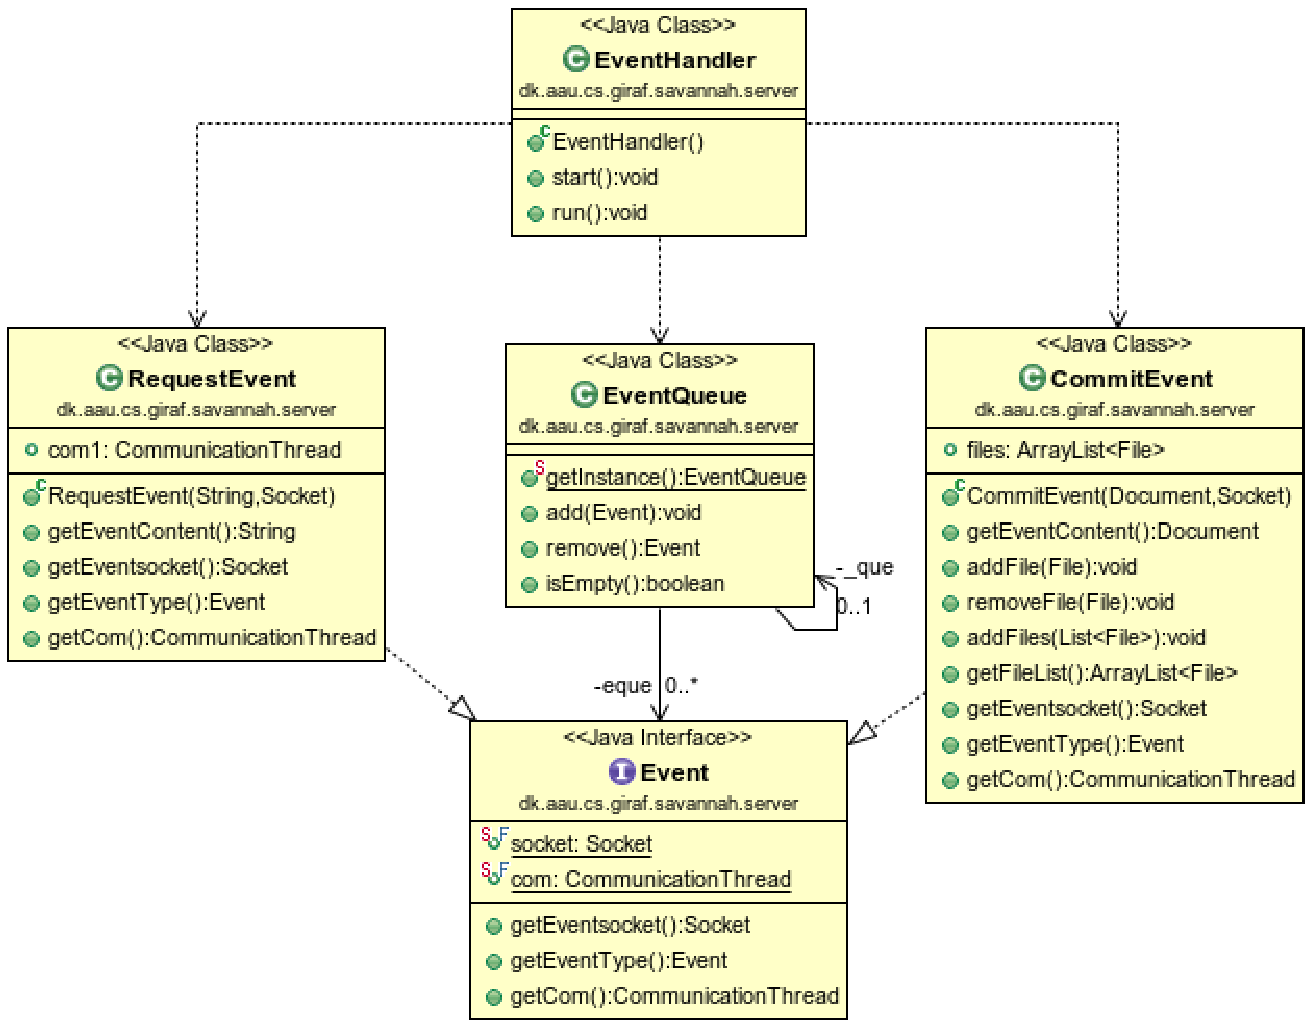
\includegraphics[scale=0.65]{images/EventQueue}
  \caption{EventQueue UML diagram.}
  \label{figure:EventUML}
\end{figure}

An event contains a reference to the socket on which the connection was made and the event content, which is either an XML document or a \code{String} containing certificates
needed to query profiles from the database.

\subsubsection{Query creation and handling}

The UML diagram in \autoref{figure:queryUML} shows the \code{EventHandler} and related classes for building SQL queries, querying the database, and building XML documents.
The \code{Eventhandler} instantiates a \code{RequestHandler} and a \code{CommitHandler}, which are responsible for handling request- or commit events.
Each of the handlers instatiate a \code{QueryBuilder} and a \code{QueryHandler}. The \code{QueryBuilder} creates SQL queries based on the event content. The queries are forwarded to the \code{QueryHandler}
that interacts with the database and, if the event is a \code{RequestEvent}, returns a \code{ResultSet} object. Finally the \code{Resultset} object is forwarded to the \code{XMLBuilder} that builds an sw6ml document,
in \code{String} form, that can be returned to the requesting party. 
\begin{figure}[H]
 \centering
  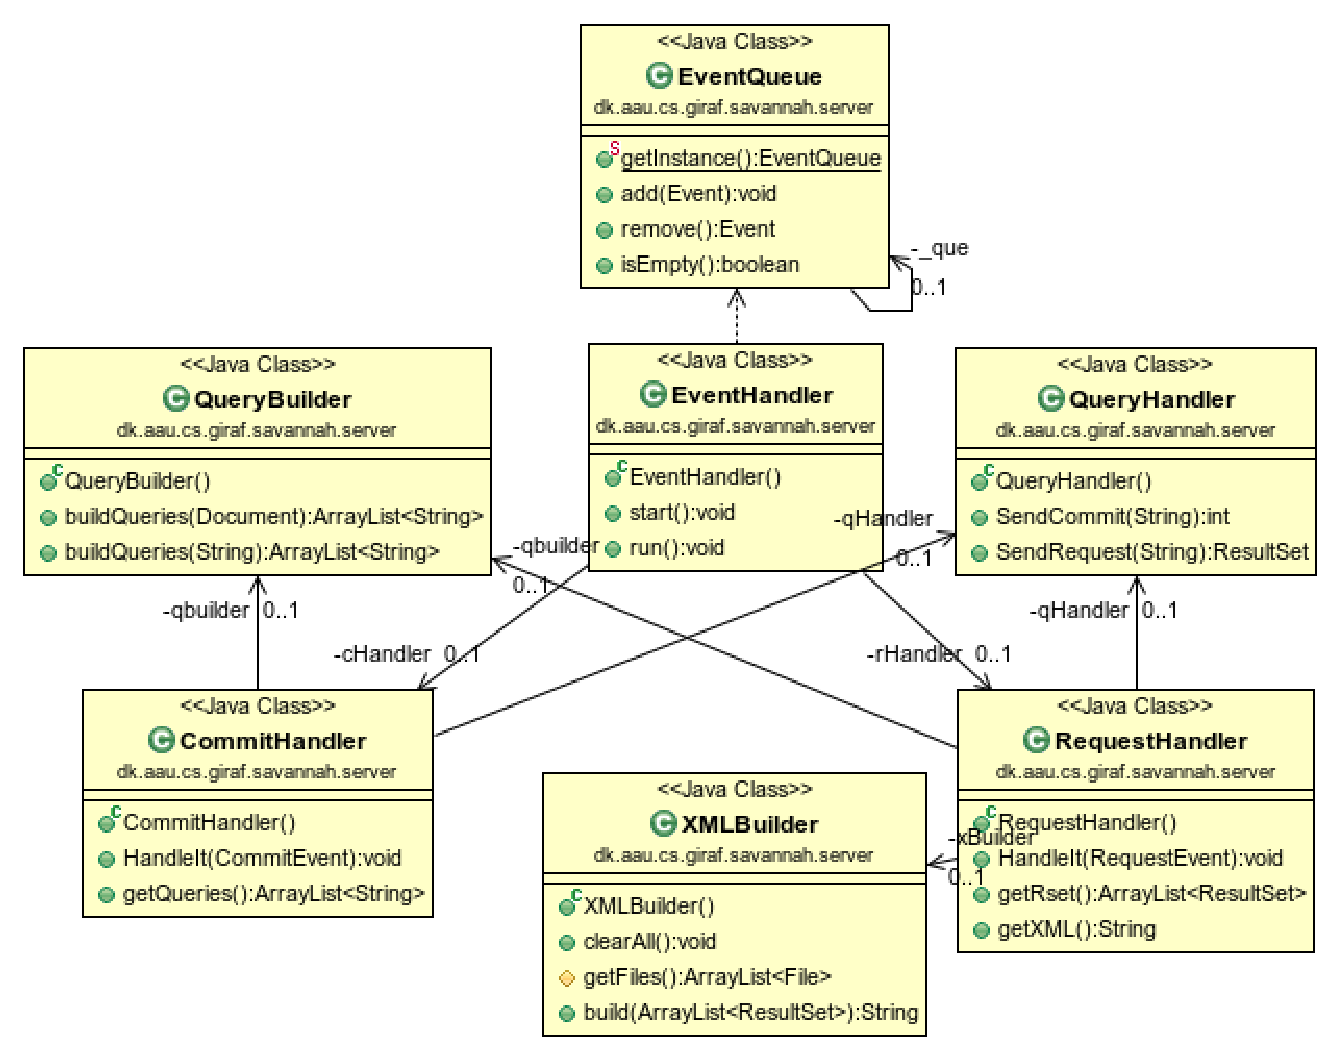
\includegraphics[scale=0.65]{images/queryhandling}
  \caption{Query handling UML diagram.}
  \label{figure:queryUML}
\end{figure}


    \subsection{Test}
	Testing on the server software has been done through JUnit test cases and big bang system tests, as well as ad hoc testing during implementation.
JUnit is a unit testing framework for java\cite{JUnit}. All tests described in this section are Dynamic white box, and has been done by the authors of the implemented software.



      \subsubsection{JUnit}
	In the \code{server} package there is a total of 10 classes which has been subjected to testing, an overview is shown in \autoref{table:qqOverview}.
The JUnit test cases column shows how many JUnit unit tests has been written for the class.

\begin{table}[H]
  \begin{center}
  \begin{tabular}{l|c|c}
    Class          & JUnit test cases & System test\\
\hline
    Event          & -                &Yes\\
    CommitEvent    & 5                &Yes\\
    RequestEvent   & -                &Yes\\
    EventHandler   & -                &Yes\\
    EventQueue     & 5                &Yes\\
    QueryBuilder   & 20               &Yes\\
    QueryHandler   & -                &Yes\\
    RequestHandler & -                &Yes\\
    CommitHandler  & -                &Yes\\
    XMLBuilder     & -                &Yes\\
  \end{tabular}
  \caption{Queue and query test overview}
  \label{table:qqOverview}
  \end{center}
\end{table}

Unit testing was not found suitable for classes all due the interdependency of other classes in the project. As en example testing the \code{XMLBuilder} with a unit test would require
a \code{ResultSet} object,the easiest way to build this is to get it from the \code{QueryHandler}, which in turn require well formed SQL queries from the \code{QueryBuilder}.
It was decided that it would be most efficient to test many of the classes during a system test. JUnit has been used to test the building of SQL queries, singleton implementation,
and that the queue is in fact Fifo. 

The code in \autoref{code:testCase} shows a JUnit test case for \code{QueryBuilder}. It verifies that the \code{QueryBuilder} properly creates an SQL query for inserting an integer value
in the \code{Media} table. Similiar test cases exists for string values and for SQL queries that update or delete rows.
Due to the implementation of \code{Querybuilder} we can cover all values and SQL query types with 9 unit tests. The remaining 11 test cases are for request queries.

\begin{Code}
\begin{lstlisting}[label=code:testCase,language=java,caption=A JUnit test case]
public void testCreateIntValue() throws Exception
{
  String xml = "<sw6ml><Media><Entry action=\"create\">" +
               "<idMedia type=\"int\">1</idMedia>" +
		"</Entry>" +
		"</Media></sw6ml>";
  doc = dom.Dominate(xml);
  ArrayList<String> one = qbuilder.buildQueries(doc);
  assertEquals("INSERT INTO Media values(1);", one.get(0) );	
}
\end{lstlisting}
\end{Code}

All classes in the \code{server} package has one or more corresponding ad hoc testing classes as well. Many of these classes are similiar in nature to the Unit tests.
They are however not automated and mostly rely on \code{System.out.println()} debuggin output, requiring a human reader. 
They also include trial and error implementation of unfamiliar technology.
In total these ad hoc testing classes total 614 lines of code



	
      \subsubsection{Other test}

\chapter{Recapitulation}
  \section{Conclusion}
  \section{Future work}
  \section{Multi project} % skal den være med

\appendix
	\chapter{Appendix}
	\section{MySQL Code}
	\label{MySQLcode}
		%appendixCreateSQL.tex
\begin{Code}
\begin{lstlisting}[language=SQL,breaklines=true, label=createAuthUsers, caption=Create AuthUsers]
  CREATE  TABLE `04`.`AuthUsers` (

  `certificate` VARCHAR(512) NOT NULL ,

  `idUser` INT NOT NULL AUTO_INCREMENT ,
  
  `aRole` INT NOT NULL,
    
  `username` VARCHAR(45) UNIQUE NOT NULL,
  
  `password` VARCHAR(45) NOT NULL,

  PRIMARY KEY (`certificate`) ,

  UNIQUE INDEX `idUser_UNIQUE` (`idUser` ASC) );
\end{lstlisting}
\end{Code}

\begin{Code}
\begin{lstlisting}[language=SQL,breaklines=true, label=createApps, caption=Create Apps, ]
  
  CREATE  TABLE `04`.`Apps` (

  `idApp` INT NOT NULL AUTO_INCREMENT,

  `name` VARCHAR(45) NOT NULL ,

  `version` VARCHAR(45) NOT NULL ,
  
  `icon` VARCHAR(45) NOT NULL,
  
  `package` VARCHAR(45) NOT NULL,
  
  `activity` VARCHAR(45) NOT NULL,

  PRIMARY KEY (`idApp`) );
\end{lstlisting}
\end{Code}

\begin{Code}
\begin{lstlisting}[language=SQL,breaklines=true, label=createTags, caption=Create Tags, ]
CREATE  TABLE `04`.`Tags` (

  `idTags` INT NOT NULL AUTO_INCREMENT,

  `caption` VARCHAR(45) NOT NULL ,

  PRIMARY KEY (`idTags`) ,

  UNIQUE INDEX `caption_UNIQUE` (`caption` ASC) );

\end{lstlisting}
\end{Code}

\begin{Code}
\begin{lstlisting}[language=SQL,breaklines=true, label=createProfile, caption=Create Profile, ]
CREATE  TABLE `04`.`Profile` (

  `idProfile` INT NOT NULL ,

  `firstname` VARCHAR(45) NOT NULL ,

  `surname` VARCHAR(45) NOT NULL ,

  `middlename` VARCHAR(45) NULL ,

  `pRole` INT NOT NULL ,

  `phone` BIGINT NOT NULL ,

  `picture` VARCHAR(45) NULL ,

  `settings` BLOB NULL ,
  
  FOREIGN KEY (`idProfile` )

  REFERENCES `04`.`AuthUsers` (`idUser` ) on delete cascade,

  PRIMARY KEY (`idProfile`) );
\end{lstlisting}
\end{Code}

\begin{Code}
\begin{lstlisting}[language=SQL,breaklines=true, label=createListOfApps, caption=Create ListOfApps, ]
CREATE  TABLE `04`.`ListOfApps` (

  `idApp` INT NOT NULL ,

  `idProfile` INT NOT NULL ,
  
  `setting` BLOB,
  
  `stats` BLOB,
  
  FOREIGN KEY (`idApp` )

  REFERENCES `04`.`Apps` (`idApp` ),
  
  FOREIGN KEY (`idProfile` )

  REFERENCES `04`.`Profile` (`idProfile` ) ON DELETE CASCADE,

  PRIMARY KEY (`idApp`,`idProfile`) );

\end{lstlisting}
\end{Code}

\begin{Code}
\begin{lstlisting}[language=SQL,breaklines=true, label=createDepartment, caption=Create Department, ]
CREATE  TABLE `04`.`Department` (

  `idDepartment` INT NOT NULL ,

  `name` VARCHAR(45) NOT NULL ,

  `address` VARCHAR(45) NOT NULL ,

  `phone` BIGINT NOT NULL ,

  `email` VARCHAR(45) NOT NULL ,
  
  FOREIGN KEY (`idDepartment` )

  REFERENCES `04`.`AuthUsers` (`idUser` ),

  PRIMARY KEY (`idDepartment`) );

\end{lstlisting}
\end{Code}

\begin{Code}
\begin{lstlisting}[language=SQL,breaklines=true, label=createHasDepartment, caption=Create HasDepartment, ]
CREATE  TABLE `04`.`HasDepartment` (

  `idProfile` INT NOT NULL ,

  `idDepartment` INT NOT NULL ,
  
  FOREIGN KEY (`idProfile` )

  REFERENCES `04`.`Profile` (`idProfile` ) ON DELETE CASCADE,

  FOREIGN KEY (`idDepartment` )

  REFERENCES `04`.`Department` (`idDepartment` ),


  PRIMARY KEY (`idProfile`, `idDepartment`) );

\end{lstlisting}
\end{Code}

\begin{Code}
\begin{lstlisting}[language=SQL,breaklines=true, label=createHasGuardian, caption=Create HasGuardian, ]
CREATE  TABLE `04`.`HasGuardian` (

  `idGuardian` INT NOT NULL ,

  `idChild` INT NOT NULL ,
  
  FOREIGN KEY (`idGuardian` )

  REFERENCES `04`.`Profile` (`idProfile` ) on delete cascade,
  
  FOREIGN KEY (`idChild` )

  REFERENCES `04`.`Profile` (`idProfile` ) on delete cascade,

  PRIMARY KEY (`idGuardian`,`idChild`) );

\end{lstlisting}
\end{Code}

\begin{Code}
\begin{lstlisting}[language=SQL,breaklines=true, label=createHasSubDepartment, caption=Create HasSubDepartment, ]
CREATE  TABLE `04`.`HasSubDepartment` (

  `idDepartment` INT NOT NULL ,

  `idSubDepartment` INT NOT NULL ,
  
  FOREIGN KEY (`idDepartment` )

  REFERENCES `04`.`Department` (`idDepartment` ),
  
  FOREIGN KEY (`idSubDepartment` )

  REFERENCES `04`.`Department` (`idDepartment` ),

  PRIMARY KEY (`idDepartment`, `idSubDepartment`) );

\end{lstlisting}
\end{Code}

\begin{Code}
\begin{lstlisting}[language=SQL,breaklines=true, label=createMedia, caption=Create Media, ]
CREATE  TABLE `04`.`Media` (

  `idMedia` INT NOT NULL AUTO_INCREMENT,

  `mPath` VARCHAR(45) NOT NULL ,

  `name` VARCHAR(45) NOT NULL ,

  `mPublic` TINYINT NOT NULL ,

  `mType` VARCHAR(45) NOT NULL ,

  `ownerID` INT NOT NULL ,
  
  FOREIGN KEY (`OwnerID` )

  REFERENCES `04`.`AuthUsers` (`idUser` )  ON DELETE CASCADE,

  PRIMARY KEY (`idMedia`) );

\end{lstlisting}
\end{Code}

\begin{Code}
\begin{lstlisting}[language=SQL,breaklines=true, label=createHasTag, caption=Create HasTag, ]
CREATE  TABLE `04`.`HasTag` (

  `idMedia` INT NOT NULL ,

  `idTag` INT NOT NULL ,
  
  FOREIGN KEY (`idMedia` )

  REFERENCES `04`.`Media` (`idMedia` ) on delete cascade,
  
  FOREIGN KEY (`idTag` )

  REFERENCES `04`.`Tags` (`idTags` ),

  PRIMARY KEY (`idMedia`, `idTag`) );

\end{lstlisting}
\end{Code}

\begin{Code}
\begin{lstlisting}[language=SQL,breaklines=true, label=createHasLink, caption=Create HasLink, ]
CREATE  TABLE `04`.`HasLink` (

  `idMedia` INT NOT NULL ,

  `idSubMedia` INT NOT NULL ,
  
  FOREIGN KEY (`idMedia` )

  REFERENCES `04`.`Media` (`idMedia` ) on delete cascade,
  
  FOREIGN KEY (`idSubMedia` )

  REFERENCES `04`.`Media` (`idMedia` ) on delete cascade,

  PRIMARY KEY (`idMedia`, `idSubMedia`) );

\end{lstlisting}
\end{Code}

\begin{Code}
\begin{lstlisting}[language=SQL,breaklines=true, label=createMediaProfileAccess, caption=Create MediaProfileAccess, ]
CREATE  TABLE `04`.`MediaProfileAccess` (

  `idProfile` INT NOT NULL ,

  `idMedia` INT NOT NULL ,
  
  FOREIGN KEY (`idProfile` )

  REFERENCES `04`.`Profile` (`idProfile` ) ON DELETE CASCADE,
  
  FOREIGN KEY (`idMedia` )

  REFERENCES `04`.`Media` (`idMedia` ) ON DELETE CASCADE,

  PRIMARY KEY (`idProfile`, `idMedia`) );

\end{lstlisting}
\end{Code}

\begin{Code}
\begin{lstlisting}[language=SQL,breaklines=true, label=createMediaDepartmentAccess, caption=Create MediaDepartmentAccess, ]
CREATE  TABLE `04`.`MediaDepartmentAccess` (

  `idDepartment` INT NOT NULL ,

  `idMedia` INT NOT NULL ,
  
  FOREIGN KEY (`idDepartment` )

  REFERENCES `04`.`Department` (`idDepartment` ),
  
  FOREIGN KEY (`idMedia` )

  REFERENCES `04`.`Media` (`idMedia` ),

  PRIMARY KEY (`idDepartment`, `idMedia`) );

\end{lstlisting}
\end{Code}

	\section{ER Diagram}
	\label{errDiagram}
		%workbenchERRdiagram.tex
\begin{figure}[ht]
	\centering
		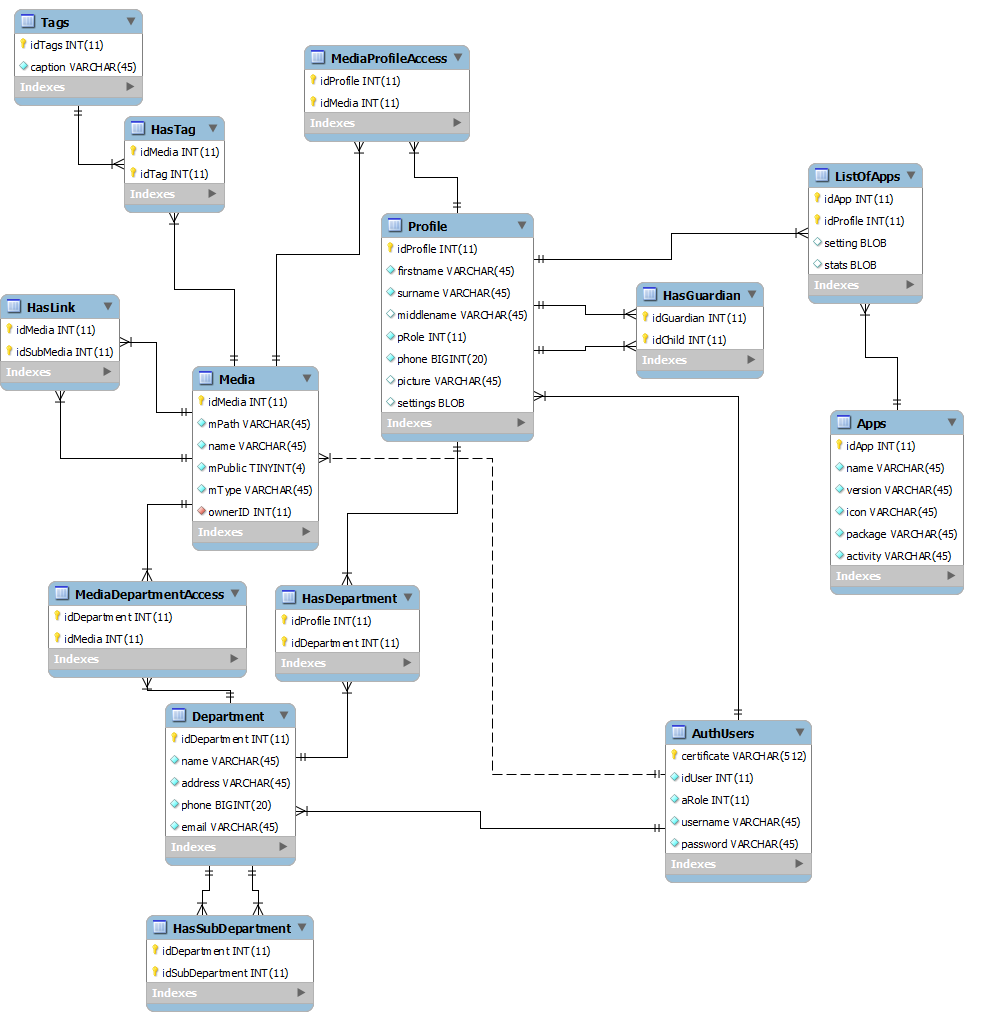
\includegraphics[width=1.00\textwidth]{images/workbenchWrong.png}
	\caption{The ERR diagram as MySQL Workbench generates it}
	\label{fig:workbenchWrong}
\end{figure}

	\section{Web interface mockups}
		%appMocks.tex


\begin{figure}[H]
	\centering
		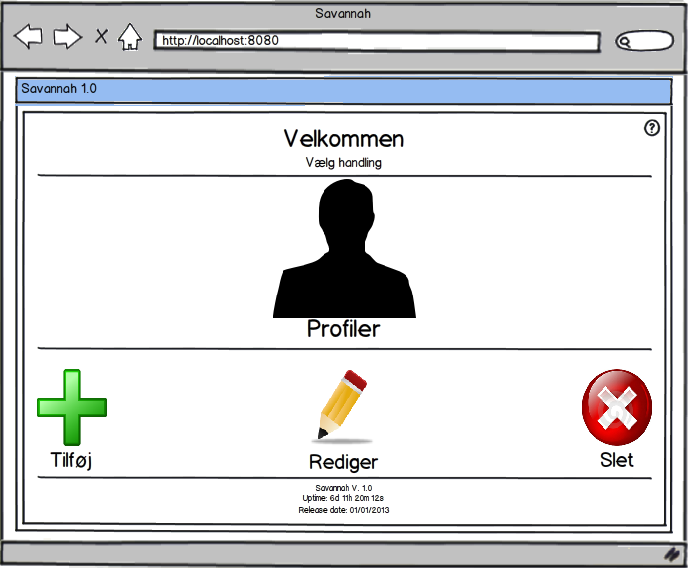
\includegraphics[width=0.60\textwidth]{images/Mocks/0-Splash.png}
		\caption{Welcome screen}
	\label{fig:0-Splash}
\end{figure}

\begin{figure}[H]
	\centering
		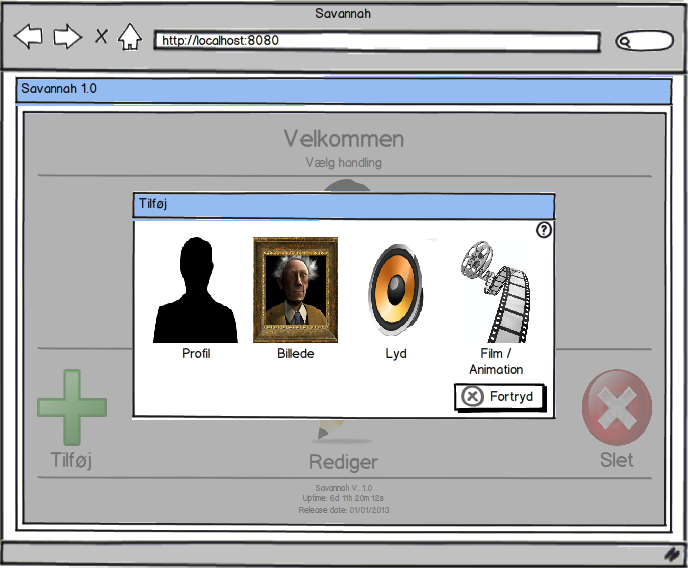
\includegraphics[width=0.60\textwidth]{images/Mocks/01-AddStuff.png}
	\caption{Add something, not logged in}
	\label{fig:01-AddStuff}
\end{figure}

\begin{figure}[H]
	\centering
		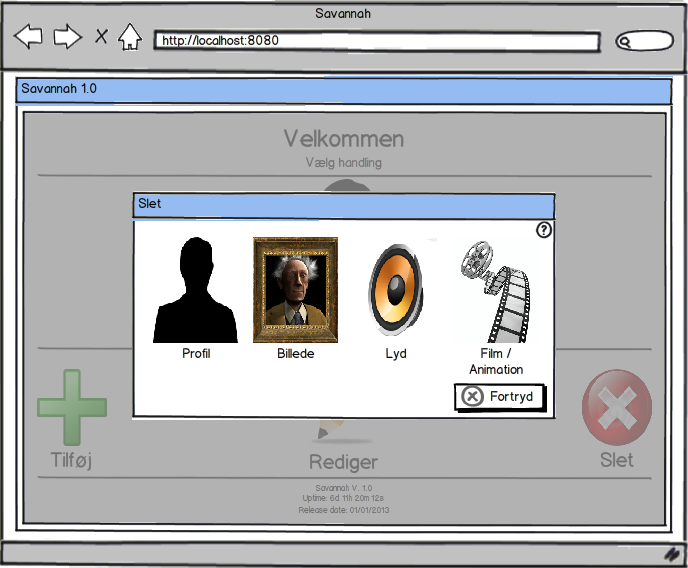
\includegraphics[width=0.60\textwidth]{images/Mocks/02-DeleteStuff.png}
	\caption{Delete something, not logged in}
	\label{fig:02-DeleteStuff}
\end{figure}

\begin{figure}[H]
	\centering
		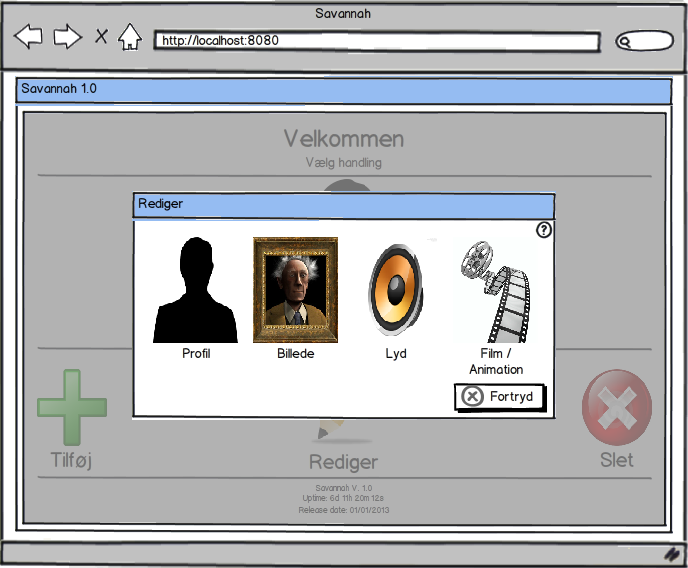
\includegraphics[width=0.60\textwidth]{images/Mocks/03-EditStuff.png}
	\caption{Edit something, not logged in}
	\label{fig:03-EditStuff}
\end{figure}

\begin{figure}[H]
	\centering
		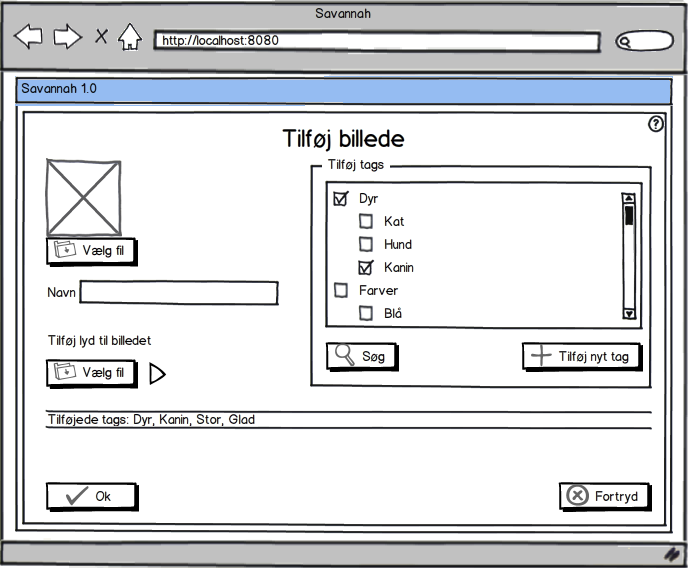
\includegraphics[width=0.60\textwidth]{images/Mocks/011-AddPicture.png}
	\caption{Add picture, not logged in}
	\label{fig:011-AddPicture}
\end{figure}

\begin{figure}[H]
	\centering
		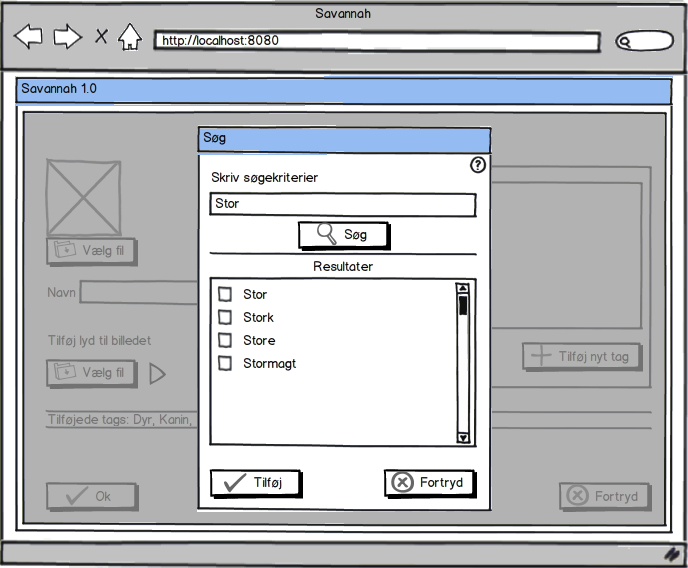
\includegraphics[width=0.60\textwidth]{images/Mocks/0111-AddPictureTags.png}
	\caption{Add picture tags}
	\label{fig:0111-AddPictureTags}
\end{figure}

\begin{figure}[H]
	\centering
		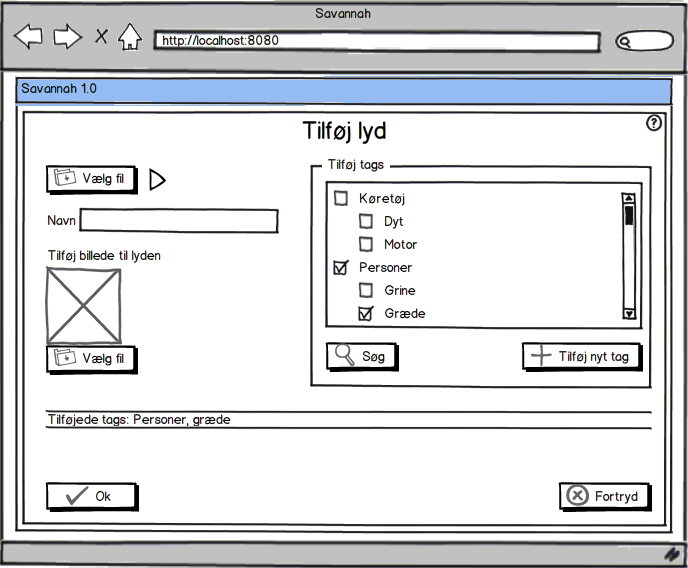
\includegraphics[width=0.60\textwidth]{images/Mocks/012-AddSound.png}
	\caption{Add sound, not logged in}
	\label{fig:012-AddSound}
\end{figure}

\begin{figure}[H]
	\centering
		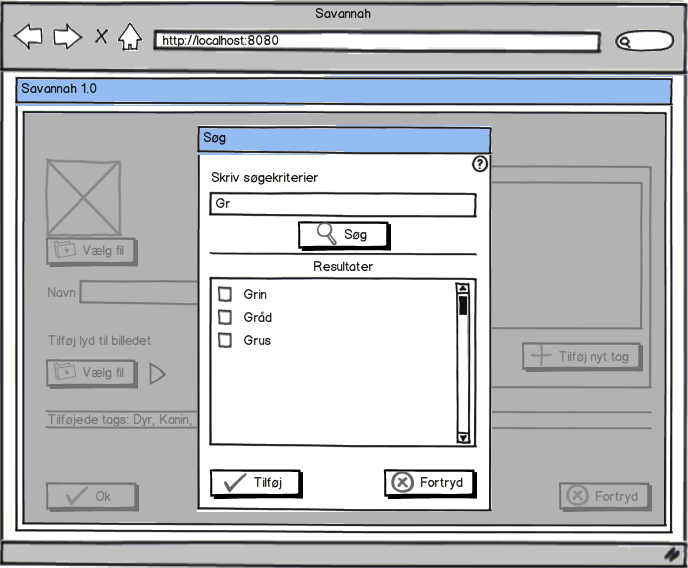
\includegraphics[width=0.60\textwidth]{images/Mocks/0121AddSoundTags.png}
	\caption{Add sound tags}
	\label{fig:0121AddSoundTags}
\end{figure}


\begin{figure}
	\centering
		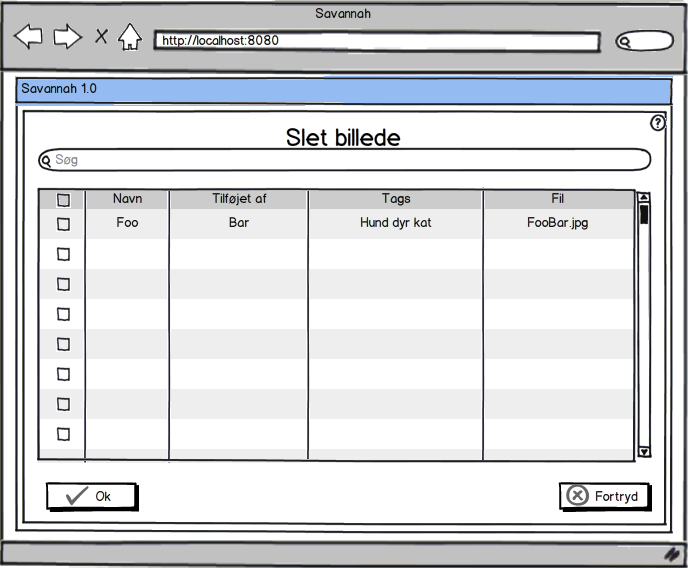
\includegraphics[width=0.60\textwidth]{images/Mocks/013-Delete.png}
	\caption{Delete something, not logged in}
	\label{fig:013-Delete}
\end{figure}

\begin{figure}[H]
	\centering
		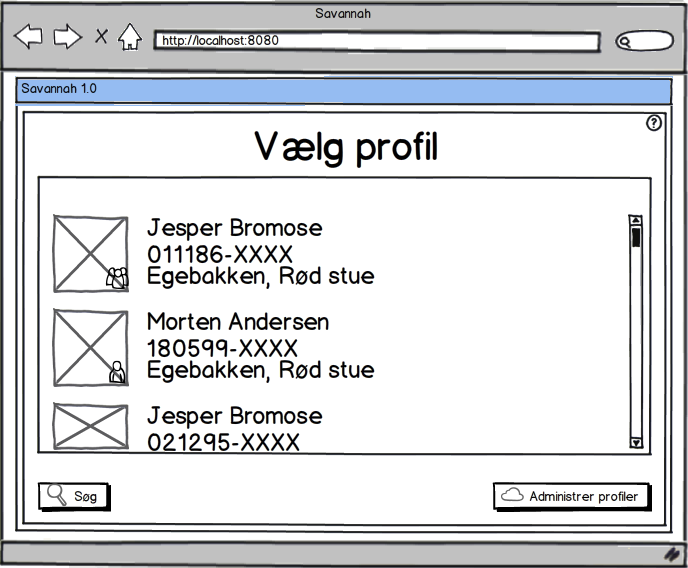
\includegraphics[width=0.60\textwidth]{images/Mocks/1-selectProfile.png}
	\caption{Select profile to login}
	\label{fig:1-selectProfile}
\end{figure}

\begin{figure}[H]
	\centering
		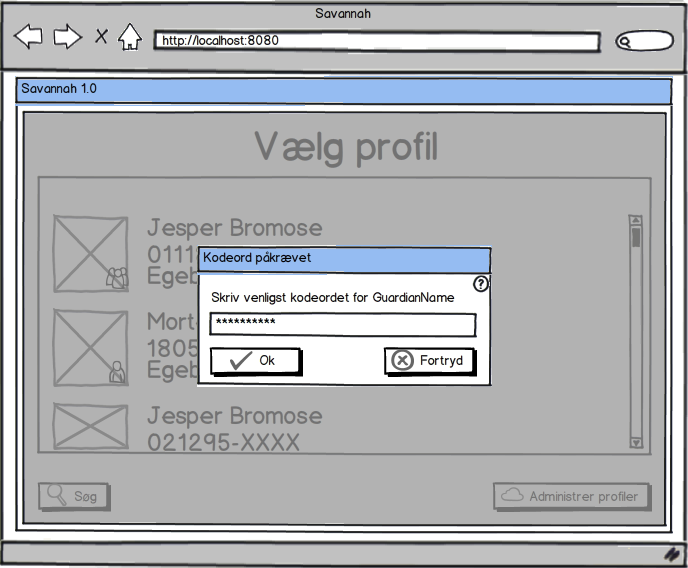
\includegraphics[width=0.60\textwidth]{images/Mocks/11-Login.png}
	\caption{Login screen}
	\label{fig:11-Login}
\end{figure}

\begin{figure}[H]
	\centering
		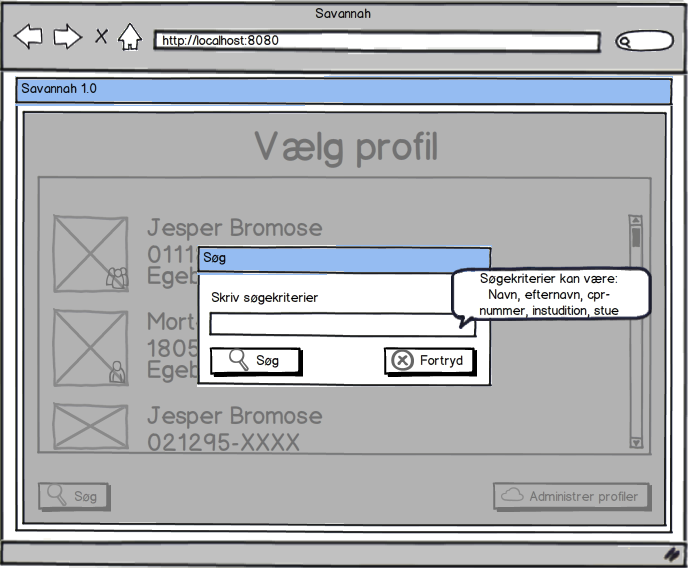
\includegraphics[width=0.60\textwidth]{images/Mocks/12-Search.png}
	\caption{Search for profile}
	\label{fig:12-Search}
\end{figure}

\begin{figure}[H]
	\centering
		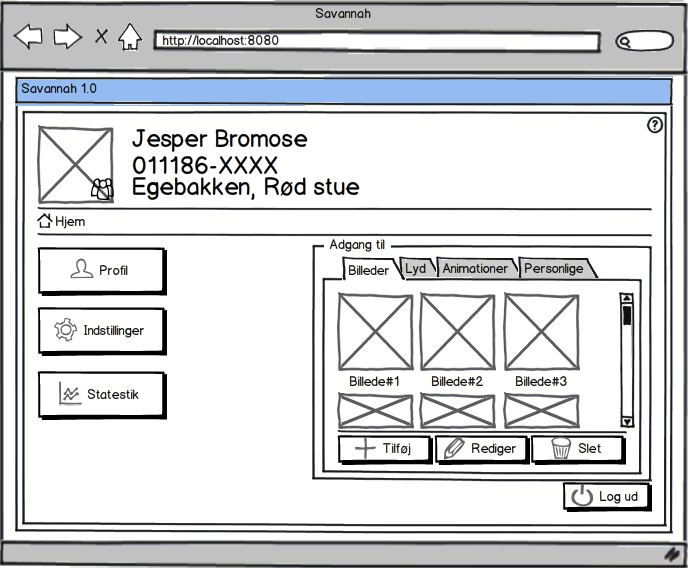
\includegraphics[width=0.60\textwidth]{images/Mocks/2-Main.png}
	\caption{Main screen}
	\label{fig:2-Main}
\end{figure}

\begin{figure}[H]
	\centering
		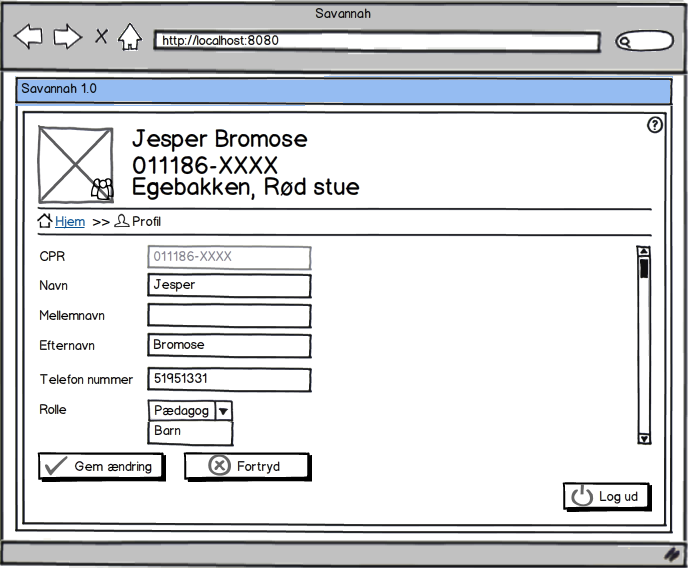
\includegraphics[width=0.60\textwidth]{images/Mocks/22-Profile.png}
	\caption{Edit profile}
	\label{fig:22-Profile}
\end{figure}

\begin{figure}[H]
	\centering
		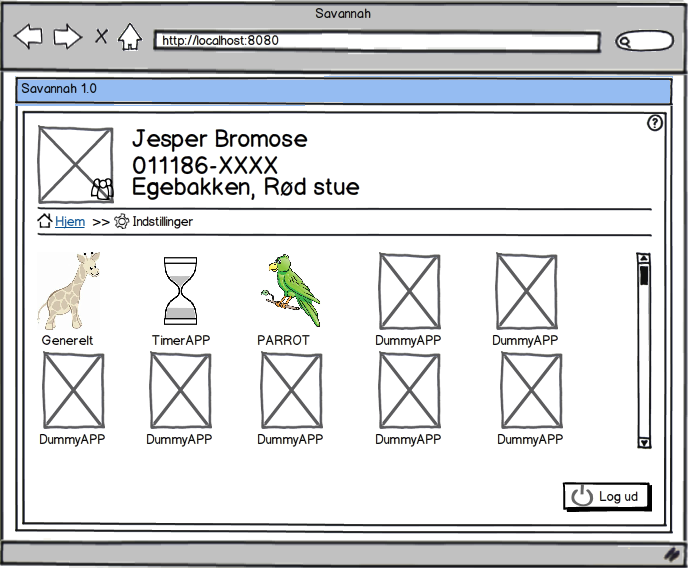
\includegraphics[width=0.60\textwidth]{images/Mocks/23-Settings.png}
	\caption{Settings}
	\label{fig:23-Settings}
\end{figure}

\begin{figure}[H]
	\centering
		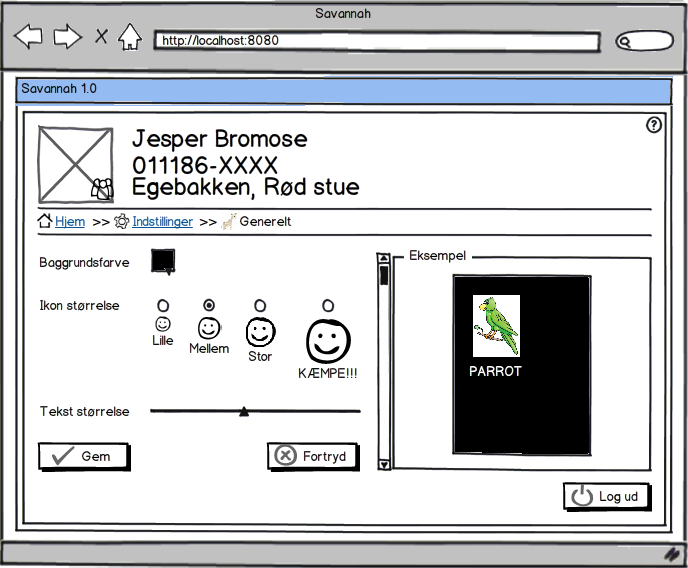
\includegraphics[width=0.60\textwidth]{images/Mocks/231-GeneralSettings.png}
	\caption{General settings}
	\label{fig:231-GeneralSettings}
\end{figure}

\begin{figure}
	\centering
		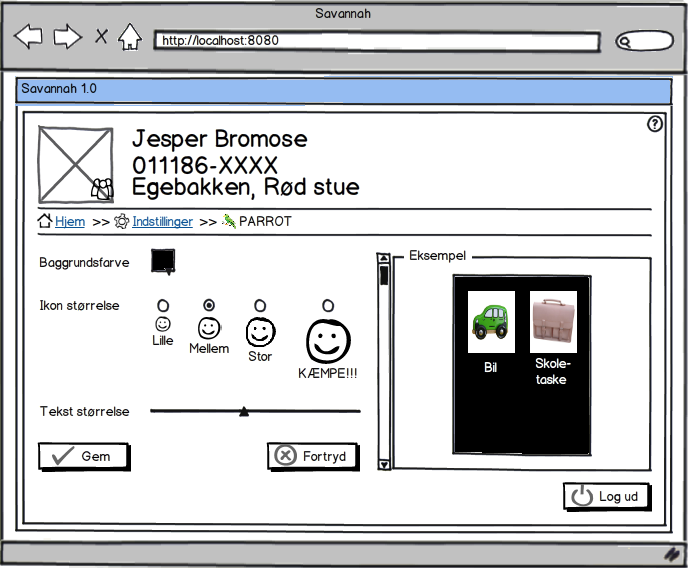
\includegraphics[width=0.60\textwidth]{images/Mocks/232-ParrotSettings.png}
	\caption{PARROT settings}
	\label{fig:232-ParrotSettings}
\end{figure}


\begin{figure}[H]
	\centering
		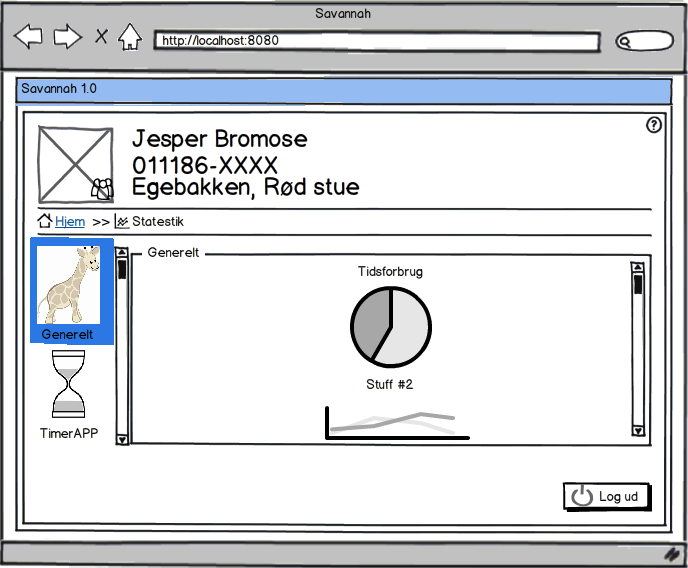
\includegraphics[width=0.60\textwidth]{images/Mocks/24-Stats.png}
	\caption{Stats}
	\label{fig:24-Stats}
\end{figure}

\begin{figure}
	\centering
		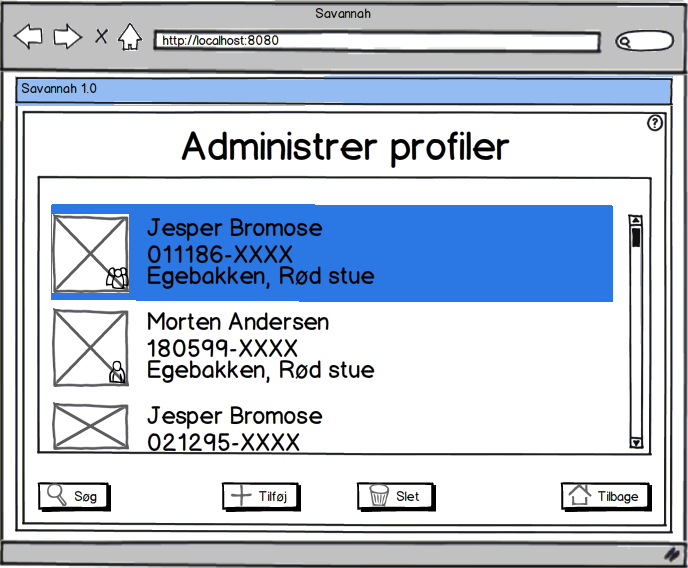
\includegraphics[width=0.60\textwidth]{images/Mocks/13-AdminProfiles.png}
	\caption{Administrate profiles}
	\label{fig:13-AdminProfiles}
\end{figure}








		\label{app:Mock}
	\section{Class Diagrams}
	\label{app:Class-diagrams}
		%appendixIOHandler.tex

\begin{figure}[H]
	\centering
		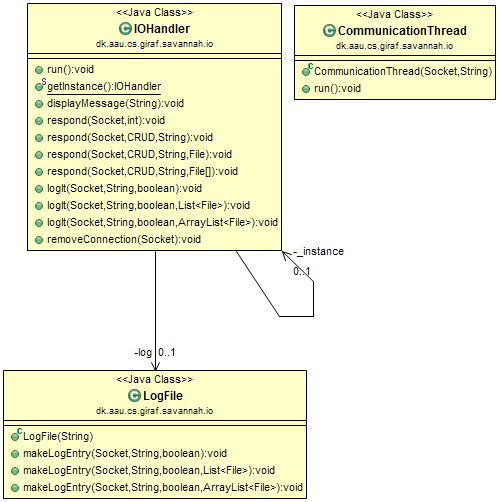
\includegraphics[scale=0.70]{images/IOHandler.PNG}
	\caption{Class-diagram of the \code{IOHandler}}
	\label{fig:app:IOHandler}
\end{figure}

\begin{figure}[H]
	\centering
		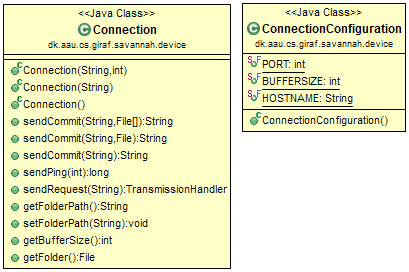
\includegraphics[scale=0.70]{images/Connection.PNG}
	\caption{Class-diagram of the \code{Connection}}
	\label{fig:app:Connection}
\end{figure}

\begin{figure}[H]
	\centering
		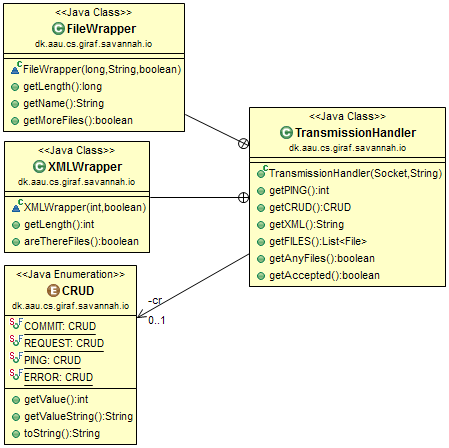
\includegraphics[scale=0.70]{images/TransmissionHandler.PNG}
	\caption{Class-diagram of the \code{TransmissionHandler}}
	\label{fig:app:TransmissionHandler}
\end{figure}
        \section{Notes from Interview}
\label{InterviewMette}
\textit{This is notes from an interview with Mette Als Andreasen, an educator at Birken in Langholt, Denmark.}

N�r tiden l�ber ud (kristian har tage et billede):\\
F�rdig - symbol\\
G� til skema - symbol\\
Taget fra boardmaker\\

Kunne v�re godt hvis man kunne s�tte egne billeder ind som start/stop symboler.\\


R�d farve $=$ nej, stop, aflyst.\\

De har s�dan et ur p� 60 minutter hvor tid tilbage er markeret med r�d, og s� bipper den lige kort n�r den er f�rdig.\\
  Det ville v�re fint hvis de kunne bruge sort/hvid til dem der ikke kan h�ndtere farver, men ogs� kan v�lge farver.\\

Stop-ur:\\
en fast timer p� 60 minutter $+$ en customizable som ikke ser helt magen til ud, som f.eks, kan v�re p� 5, 10 eller 15 minutter for en hel cirkel.\\

timeglas:\\
skift farve p� timeglassene, men ikke n�dvendigvis g�re dem st�rre. Kombinere med mere/mindre sand. Eventuelt kombinere med et lille digitalt ur, til dem der har brug for det, skal kunne sl�es til og fra.\\

Dags-plan:\\
ikke s�rlig relevant til de helt sm� og ikke s�rligt velfungerende b�rn. Men kunne v�re rigtig godt til de lidt �ldre.\\
   En plan g�r oppefra og ned, og hvis der s� skal specificeres noget ud til aktiviteterne, s� er det fra venstre mod h�jre ud fra det nedadg�ende skema.\\

Til parrot:\\
Godt med rigtige billeder af tingene, som p�dagogerne selv kan tage, eventuelt ogs� af aktiviteter, s� pedagogerne kan have billeder af aktiviter som de kan liste efter skeamet.\\

Der var mange skemaer rundt omkring, og der henviser det sidste billede i r�kken til n�ste skema, som h�nger f.eks. p� badev�relset eller i garderoben.
\begin{figure}%
	\begin{center}
	\includegraphics[width=\textwidth]{input/appendices/invitationToUsabilityTest.pdf}
	\end{center}
\caption{Invitation sent to the test persons of the usability test.}%
\label{appendice:usabilitytest}%
\end{figure}
\bibliographystyle{plainnat}
\bibliography{bib}

\appendix

\end{document}
